

\chapter{强化学习的心理学} \label{chap:chap11}

在前面的章节中,我们仅从计算方面考虑就提出了算法的设想。
在本章中,我们将从另一种视角来看待这些算法:心理学及其对动物学习的研究视角。
本章的目的首先是,讨论强化学习的理念和算法如何与心理学家关于动物学习的发现相对应;其次是,解释强化学习对动物学习研究的影响。
强化学习提供的明确形式系统化了任务、回报和算法,这对于理解实验数据、提出新实验的种类以及指向可能需要操控和测量的关键因素,都是极其有用的。
强化学习核心的长期优化回报的理念,正在帮助我们理解动物学习和行为中一些令人困惑的特征。


强化学习与心理学理论之间的一些对应关系并不令人惊讶,因为强化学习的发展受到了心理学学习理论的启发。
然而,在本书中,我们从人工智能研究者或工程师的角度,探讨了理想化的情况,旨在通过高效算法解决计算问题,而不是详细地复制或解释动物如何学习。
因此,我们描述的一些对应关系将各自领域中独立产生的想法联系起来。
我们认为这些联系点特别有意义,因为它们揭示了无论是通过人工系统还是自然系统学习都至关重要的计算原理。


在大多数情况下,我们描述的是强化学习与学习理论之间的对应关系,这些理论旨在解释像老鼠、鸽子和兔子等动物在受控实验中如何学习。
20世纪进行过成千上万的此类实验,许多至今仍在进行。
虽然有时这些实验被认为与心理学的更广泛问题无关,但它们探究了动物学习的微妙特性,常常是由精确的理论问题驱动的。
随着心理学的重点转向行为的认知方面,即思维和推理等心理过程,动物学习实验在心理学中的作用逐渐减弱。
然而,这些实验发现的学习原则是动物王国中普遍且基本的,在设计人工学习系统时不应被忽视。
此外,正如我们将看到的,有些认知处理方面与强化学习提供的计算视角自然地联系在一起。


本章的最后一节包含了与我们讨论的联系以及我们忽略的联系相关的参考文献。
我们希望本章能鼓励读者更深入地探讨所有这些联系。
此外,这一节还讨论了强化学习中使用的术语与心理学中的术语之间的关系。
强化学习中使用的许多术语和短语借鉴了动物学习理论中的概念,但这些术语和短语在计算/工程学中的含义并不总是与它们在心理学中的含义一致。


\section{预测和控制}


我们在本书中描述的算法大致可分为两大类:预测算法和控制算法。
这些类别自然地源于第三章提出的强化学习问题的解决方法。
在许多方面,这些类别分别对应于心理学家广泛研究的学习类别:经典条件反射(或巴甫洛夫式条件反射)和操作条件反射(或工具性条件反射)。
这些对应关系并非完全偶然,因为心理学对强化学习有影响,但它们仍然引人注目,因为它们连接了来自不同目标的想法。


本书介绍的预测算法用于估计依赖于代理环境特征如何在未来展开的数量。
我们特别关注于估计代理在与其环境交互过程中,未来可能获得的回报数量。
在这一角色中,预测算法是策略评估算法,是用于改进策略的算法的核心组成部分。
但预测算法不仅限于预测未来的回报;他们还可以预测环境的任何特征\cite{modayil2014prediction}。
预测算法和经典条件反射之间的对应关系在于它们共同预测即将到来的刺激这一特性,无论这些刺激是否是奖励(或惩罚)的。


在操作性条件反射(或工具性条件反射)实验中的情况有所不同。
在这里,实验装置被设置为根据动物的行为给予它喜欢的东西(奖励)或不喜欢的东西(惩罚)。
动物通过学习增加产生被奖励行为的倾向,并减少产生被惩罚行为的倾向。
强化刺激被认为依赖于动物的行为,而在经典条件反射中则不是(尽管在经典条件反射实验中完全去除行为依赖性是困难的)。
操作性条件反射实验就像我们在第一章中简要讨论过的那些启发\textit{桑代克}效应定律的实验。
控制是这种学习形式的核心,对应于强化学习中策略改进算法的运作。


将经典条件反射视为预测,将工具性条件反射视为控制,这是将我们的强化学习计算视角与动物学习联系起来的起点,但实际上情况比这更复杂。
经典条件反射不仅仅涉及预测;它也涉及行动,因此也是一种控制模式,有时被称为巴甫洛夫式控制。
此外,经典条件反射和工具性条件反射以有趣的方式相互作用,在大多数实验情况下,两种学习方式都可能参与其中。
尽管存在这些复杂情况,将经典/工具性区分与预测/控制区分对齐,是在将强化学习与动物学习联系起来时一个方便的初步近似方法。


在心理学中,术语“强化”用于描述经典条件反射和工具性条件反射中的学习。
最初它只指行为模式的加强,但现在也经常用于描述行为模式的削弱。
被认为是导致行为变化的刺激称为“强化物”,无论它是否依赖于动物先前的行为。
在本章的末尾,我们将更详细地讨论这个术语,以及它与机器学习中使用的术语的关系。


\section{经典条件反射} \label{sec:classical_conditioning}

在研究消化系统的活动时,著名的俄罗斯生理学家\textit{伊万$\cdot$巴甫洛夫}发现,动物对某些触发刺激的天生反应可以被其他完全不相关的刺激触发。
他的实验对象是经过小手术的狗,这样可以准确测量它们唾液反射的强度。
在一个案例中,他描述了,狗在大多数情况下不会流口水,但在被给予食物约5秒后,在接下来的几秒内会分泌大约6滴唾液。
在多次重复另一个与食物无关的刺激(在本例中是节拍器的声音)在引入食物之前的几秒钟后,这只狗在听到节拍器的声音时像对食物那样流口水。
“因此,唾液腺的活动被声音的刺激所引发,这是一种与食物完全不同的刺激”。
巴甫洛夫总结了这一发现的重要性,写道:


很明显,在自然条件下,正常动物不仅必须对自身带来直接好处或伤害的刺激作出反应,而且还必须对其他物理或化学因素作出反应——如声波,光波等,这些因素本身只发出这些刺激的接近信号;
虽然猛兽的声音和影像本身对较小的动物并不有害,但它的牙齿和爪子却是有害的。


将新刺激与先天反射联系起来的这种方式现在被称为经典条件反射(或巴甫洛夫式条件反射)。
\textit{巴甫洛夫}(或者更确切地说,他的译者)将先天反应(例如,在他前述示例中的唾液分泌)称为“\textit{无条件反应}”,将其自然触发刺激(例如食物)称为“\textit{无条件刺激}”,而将由预测刺激触发的新反应(例如这里也是唾液分泌)称为“\textit{条件反应}”。
一种最初是中性的刺激,意思是它通常不会引起强烈反应(例如节拍器的声音),随着动物学习到它预示着\textit{无条件刺激}的出现而产生\textit{条件反应},这种刺激就成为“\textit{条件刺激}”。
这些术语仍然用于描述经典条件反射实验(尽管更好的翻译应该是“条件的”和“无条件的”,而不是“条件反射的”和“无条件反射的”)。
\textit{无条件刺激}被称为强化物,因为它强化了动物在面对\textit{条件刺激}时产生\textit{条件反应}的行为。


右图显示了经典条件反射实验中两种常见类型的刺激安排。
在延迟条件反射中,\textit{条件刺激}在\textit{刺激间隔}期间持续存在,即从\textit{条件刺激}开始到\textit{非条件刺激}(\textit{无条件刺激})开始的时间间隔(在此处常见版本中,\textit{条件刺激}在\textit{无条件刺激}结束时结束)。
在痕迹条件反射中,\textit{无条件刺激}在\textit{条件刺激}结束后开始,\textit{条件刺激}结束与\textit{无条件刺激}开始之间的时间间隔称为痕迹间隔。


\begin{figure}[!htb]
	\centering
	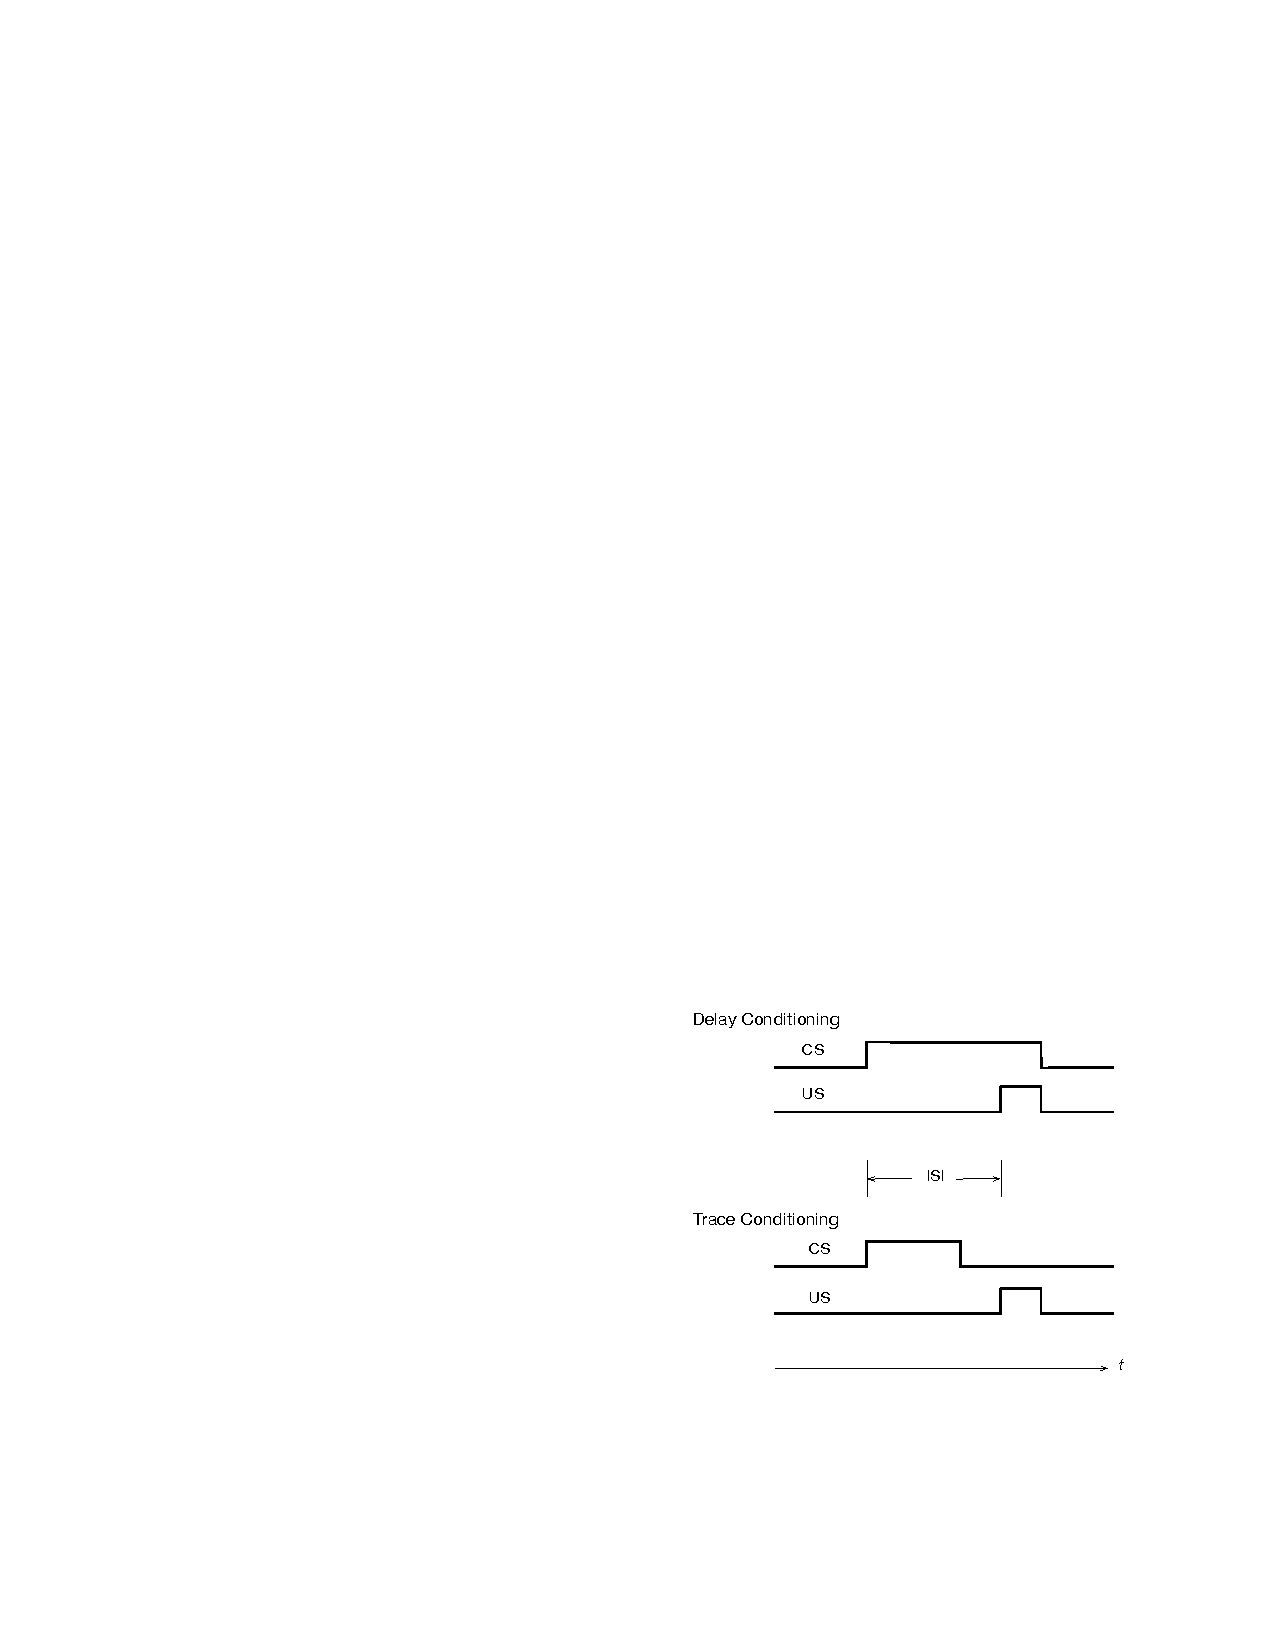
\includegraphics[width=0.5\linewidth]{chap11/fig_11_0}
	\caption{  \label{fig:11_0}}
\end{figure}


\textit{巴甫洛夫}的狗对节拍器声音流口水只是经典条件反射的一个例子,这种现象已经在许多动物种类的多种反应系统中进行了深入研究。
\textit{无条件反应}通常在某种程度上是准备性的,比如\textit{巴甫洛夫}的狗的流口水,或者是保护性的,比如眼睛对刺激物的眨眼反应,或者看到捕食者时的冻结反应。
通过一系列试验经历\textit{条件刺激}与\textit{无条件刺激}的预测关系,使得动物学会了\textit{条件刺激}预测\textit{无条件刺激},因此动物可以用\textit{条件反应}来对\textit{条件刺激}做出反应,以准备迎接或保护自己免受预测到的\textit{无条件刺激}的影响。
一些\textit{条件反应}与\textit{无条件反应}类似,但开始得更早,并在某些方面有所不同,从而提高了它们的有效性。
例如,在一种经过深入研究的实验中,一个音调\textit{条件刺激}可靠地预测了兔子眼睛中的一股空气,引发了无条件反应,包括保护性内膜(瞬膜)的关闭。
在一轮或多轮试验后,该音调开始触发条件反应,即膜关闭,它在空气吹起前开始,最终时间安排得恰到好处,使得膜的最大闭合恰好发生在空气吹起的时刻。
这个条件反应由于在空气吹起之前提前启动,并且时间安排得当,提供了比简单地作为对刺激性\textit{无条件刺激}的反应而启动关闭更好的保护。
通过学习刺激之间的预测关系来预见重要事件的能力是如此有益,以至于在整个动物王国中广泛存在。


\subsection{阻塞和高阶条件反射} \label{sec:blocking_higher_order}

在实验中已经观察到经典条件反射的许多有趣性质。
除了\textit{条件反射}的预期性质之外,在经典条件反射模型的发展中,两个广泛观察到的特性得到了显着体现:阻塞和高阶条件反射。
阻塞发生在一个潜在的\textit{条件刺激}与之前用于使动物产生\textit{条件反射}的另一个\textit{条件刺激}一起出现时,动物未能学习该\textit{条件反射}。
例如,在涉及兔子第三眼睑条件反射的阻塞实验的第一阶段,兔子首先通过音调\textit{条件刺激}和空气喷射 \textit{非条件刺激}的结合来条件化,产生预期空气喷射的第三眼睑关闭\textit{条件反射}。
实验的第二阶段包括额外的试验,其中第二个刺激(例如光)被添加到音调中以形成复合音调/光\textit{条件刺激},然后是相同的空气喷射 \textit{非条件刺激}。
在实验的第三阶段,仅第二个刺激(即光)被呈现给兔子,以查看兔子是否已经学会了用\textit{条件反射}对其作出反应。
结果表明,兔子对光的反应产生了很少或没有\textit{条件反射}:对光的学习已经被先前对音调的学习所阻塞。
这样的阻塞结果挑战了条件反射只依赖于简单的时间连续性的观点,即条件反射的必要和充分条件是\textit{非条件刺激}经常在时间上紧跟\textit{条件刺激}。
在下一节中,我们将描述\textit{雷斯科拉-瓦格纳模型}\cite{rescorla1972theory},该模型为阻塞提供了全面的解释。



当先前条件化的\textit{条件刺激}充当\textit{非条件刺激}来条件化另一个最初中性的刺激时,就会发生高阶条件化。
如上所述,巴甫洛夫描述了一个实验,在这个实验中,他的助手首先条件化一只狗,让它随着节拍器的声音流涎,节拍器可以预测食物的味道。
在这个调节阶段之后,进行了许多试验,一块黑色方块(狗最初对此无动于衷)被放在狗的视线中,然后是节拍器的声音,而不是食物。
在仅仅十次试验后,这只狗只在看到黑色方块时就开始流口水,尽管事实上,看到它之后从来没有得到过食物。
节拍器的声音本身就像一个\textit{非条件刺激},将流涎的\textit{条件反射}条件化为黑色方块\textit{条件刺激}。
这是二阶条件反射。如果黑色方块被用作\textit{非条件刺激}来建立另一个中性\textit{条件刺激}的唾液\textit{条件反射},那么它将是三阶条件反射,依此类推。高阶条件反射很难证明,特别是在二阶以上,部分原因是高阶增强物由于在高阶条件反射试验中没有被原\textit{非条件刺激}反复遵循而失去了增强价值。
但是在正确的条件下,例如将一阶试验与高阶试验混合或通过提供一般的激励刺激,可以证明二阶以上的高阶条件反射。
正如我们在下面所描述的,经典条件反射的\textit{时间差分}模型使用了自举思想,这是我们的方法的核心,以扩展\textit{雷斯科拉-瓦格纳模型}对阻塞的描述,以包括\textit{条件反射}的预期性质和高阶条件反射。


高阶工具性条件反射也会发生。
在这种情况下,持续预测初级强化的刺激本身就变成了强化剂,如果通过进化将其奖励或惩罚的品质建立在动物体内,则强化是主要的。
预测刺激成为二级增强剂,或者更一般地说,是高阶或条件性增强剂--当预测的增强刺激本身是二级或甚至更高阶的增强剂时,后者是更好的术语。
条件性强化剂提供条件性强化:条件性奖励或条件性惩罚。
条件性强化就像初级强化一样,增加动物产生导致条件性奖励的行为的倾向,并减少动物产生导致条件性惩罚的行为的倾向。
(请参阅本章末尾的评论,解释我们的术语有时与心理学中使用的术语有何不同。)



条件性强化是一个关键现象,它解释了为什么我们为条件性强化货币工作,而条件性强化货币的价值完全来自于拥有它所预测的东西。
在第13.5节描述的\textit{行动者}-\textit{评论家}方法(并在第15.7节和第15.8节的神经科学背景下进行了讨论)中,\textit{评论家}使用\textit{时间差分}方法来评估\textit{行动者}的政策,其价值估计为\textit{行动者}提供了条件性强化,从而使\textit{行动者}能够改进其政策。
这种更高阶的工具性条件作用的类似物有助于解决第1.7节中提到的信贷分配问题,因为当主要奖励信号延迟时,评论家会对\textit{行动者}进行即时强化。
我们将在下面的第14.4节中对此进行更多讨论。


\subsection{雷斯科拉-瓦格纳模型} \label{sec:rescorla_wagner}

\textit{雷斯科拉}和\textit{瓦格纳}创建模型主要是为了解释阻塞现象。
\textit{雷斯科拉-瓦格纳模型}的核心思想是,动物只有在事件违反其预期时才会学习,换句话说,只有当动物感到惊讶时(尽管不一定意味着任何有意识的期望或情绪)。
我们首先使用\textit{雷斯科拉}和\textit{瓦格纳}的术语和符号来介绍模型,然后再转向我们用来描述\textit{时间差分}模型的术语和符号。


以下是\textit{雷斯科拉}和\textit{瓦格纳}描述他们模型的方式。
该模型调整复合\textit{条件刺激}的每个成分刺激的“关联强度”,这是一个表示该成分预测\textit{非条件刺激}的强度或可靠性的数字。
当在经典条件反射试验中呈现由多个成分刺激组成的复合 \textit{条件刺激}时,每个成分刺激的关联强度的变化方式取决于与整个刺激复合体相关的关联强度,称为“聚合关联强度”,而不仅仅取决于每个成分本身的关联强度。


\textit{雷斯科拉}和\textit{瓦格纳}考虑了一种复合\textit{条件刺激} AX,由组成刺激A和X组成,其中动物可能已经经历了刺激A,而刺激X对动物来说可能是新的。设$V_A$,$V_X$和$V_{AX}$分别表示刺激A,X和合AX的结合强度。
假设在试验中,复合\textit{条件刺激} AX后面跟着一个\textit{非条件刺激},我们将其标记为刺激Y。
然后刺激组成部分的关联强度根据以下表达式变化:

\begin{equation}
	\Delta V_A = \alpha_A \beta_Y
	(R_Y - V_{AX})
\end{equation}


\begin{equation}
	\Delta V_X = 
	\alpha_X \beta_Y
	(R_Y - V_{AX})
\end{equation}

其中$\alpha_{\mathrm{A}} \beta_{\mathrm{Y}}$和$\alpha_{\mathrm{X}} \beta_{\mathrm{Y}}$是步长参数,取决于\textit{条件刺激}分量和\textit{非条件刺激}的特性,$R_{\mathrm{Y}}$是\textit{非条件刺激}Y可以支持的关联强度的渐近水平。
(\textit{雷斯科拉}和\textit{瓦格纳}在这里使用R代替$\lambda$,但我们使用R是为了避免与我们使用$\lambda$混淆,因为我们通常认为这是奖励信号的大小,但需要注意的是,经典条件反射中的\textit{非条件刺激}不一定是奖励或惩罚。)该模型的一个关键假设是总关联强度$V_{\mathrm{AX}}$等于$V_{\mathrm{A}}$+$V_{\mathrm{X}}$。
由这些$\Delta s$改变的关联强度变化成为下一次试验开始时的关联强度。


为了完整,该模型需要一种响应生成机制,这是一种将$V_{\mathrm{s}}$值映射到\textit{条件反射}的方法。
因为这种映射将取决于实验情况的细节,所以\textit{雷斯科拉}和\textit{瓦格纳}没有指定映射,而是简单地假设较大的$V_{\mathrm{s}}$会产生更强或更可能的\textit{条件反射},并且负$V_{\mathrm{s}}$意味着不会有\textit{条件反射}。



\textit{雷斯科拉-瓦格纳模型}以一种解释阻塞的方式解释了\textit{条件反射}的获取方式。
只要刺激复合物的总关联强度$V_{\mathrm{AX}}$低于\textit{非条件刺激}Y可以支持的关联强度$R_{\mathrm{Y}}$的渐近水平,预测误差$R_{\mathrm{Y}}$-$V_{\mathrm{AX}}$为正值。
这意味着在连续的试验中,组成刺激的各部分$V_{\mathrm{A}}$和$V_{\mathrm{X}}$的关联强度会增加,直到总关联强度$V_{\mathrm{AX}}$等于$R_{\mathrm{Y}}$,此时关联强度停止变化(除非\textit{非条件刺激}改变)当一个新成分被加入到已经使动物形成条件反射的复合物已经调理过的复合\textit{条件刺激}中时,通过增强复合物进行的进一步条件反射训练几乎不会增加新加入的\textit{条件刺激}成分的关联强度,因为误差已经减小到零或低值。
\textit{非条件刺激}的发生几乎已经被完美地预测到了,因此新的\textit{条件刺激}组件几乎没有引入错误或惊讶。先前的学习阻碍了对新组件的学习。



为了从\textit{雷斯科拉}和\textit{瓦格纳}的模型过渡到经典条件反射的\textit{时间差分}模型(我们称之为\textit{时间差分}模型),我们根据本书中使用的概念重新构建了他们的模型。
具体来说,我们将用于学习的符号与线性函数近似(第9.4节)相匹配,并将条件反射过程视为根据试验中呈现的复合\textit{条件刺激}预测试验中\textit{非条件刺激}的“强度”,其中\textit{非条件刺激}Y的大小是如上所述的\textit{雷斯科拉-瓦格纳模型}的$R_{\mathrm{Y}}$。
我们还引入了状态。因为\textit{雷斯科拉-瓦格纳模型}是一个试验级模型,这意味着它处理了从试验到试验的关联强度如何变化,而不考虑试验内部和试验之间发生的任何细节,我们不必考虑在试验期间状态如何变化,直到我们在下一节。
相反,在这里,我们简单地将状态视为根据试验中存在的组件\textit{条件刺激}的集合来标记试验的一种方式。


因此,假设试验类型或状态s由一个实值特征向量$\mathbf{x}(s)=\left(x_{1}(s), x_{2}(s), \ldots, x_{d}(s)\right)^{\top}$描述,其中如果组成CS的第i个成分$CS_{\mathrm{i}}$在试验中存在,则xi(s) = 1,否则为0。
然后,如果关联强度的d维向量为w,则试验类型s的总关联强度为

\begin{equation}\label{key}
	v(s, \textbf{w}) = 
	w^T x(s).
\end{equation}
这对应于强化学习中的价值估计,我们认为它是\textit{非条件刺激}的预测。

现在暂时令t表示完整试验的次数,而不是它作为时间步长的通常含义(当我们将其扩展到下面的\textit{时间差分}模型时,我们恢复到t的通常含义),并假设$S_{\mathrm{t}}$是对应于试验t的状态。
条件试验t将关联强度向量$w_{\mathrm{t}}$更新为$w_{\mathrm{t+1}}$,如下所示:

\begin{equation}\label{key}
	w_{t+1} = w_t + \alpha \delta_t x(S_t),
\end{equation}

其中$\alpha$是步长参数,因为这里我们描述的是\textit{雷斯科拉-瓦格纳模型}——$\delta_t $是预测误差

\begin{equation}\label{key}
	\delta = R_t - v (S_t, w_t).
\end{equation}


$R_{\mathrm{t}}$是试验t预测的目标,即\textit{非条件刺激}的强度,或者用\textit{雷斯科拉}和\textit{瓦格纳}的话说,是\textit{非条件刺激}在试验中可以支持的联合强度。
请注意,由于(14.2)中的因子$\ x(S_t)$,因此只有试验中存在的\textit{条件刺激}组件的关联强度才能作为该试验的结果进行调整。
你可以将预测误差视为惊喜的衡量标准,将总关联强度视为动物的期望,当它与\textit{非条件刺激}的目标幅度不匹配时,就会被违反。


从机器学习的角度来看,\textit{雷斯科拉-瓦格纳模型}是一种纠错监督学习规则。它本质上与最小均方(LMS)或 Widrow-Hoff 学习规则(Widrow 和 Hoff,1960 年)相同,该规则找出使所有误差的平方的平均值尽可能接近于零的权重——这里是关联强度。
这是一种广泛应用于工程和科学领域的“曲线拟合”或回归算法(见第 9.4 节)。




\textit{雷斯科拉-瓦格纳模型}在动物学习理论的历史上是非常重要的,因为它表明一个“机械”理论可以解释关于阻塞的主要事实,而不需要诉诸更复杂的认知理论,例如,动物明确认识到另一个刺激成分已被添加,然后回溯其短期记忆重新评估与 \textit{非条件刺激}相关的预测关系。
\textit{雷斯科拉-瓦格纳模型}展示了如何通过简单的方式调整传统的邻近性学习理论(即刺激的时间邻近性是学习的必要和充分条件)来解释阻碍效应(Moore 和 Schmajuk,2008)。


\textit{雷斯科拉-瓦格纳模型}提供了经典条件反射的阻塞和其他一些特征的简单说明,但它不是经典条件反射的完整或完美模型。
不同的理论解释了各种其他观察到的效应,并且在理解经典条件反射的许多微妙之处方面仍在取得进展。
我们接下来描述的\textit{时间差分}模型虽然也不是经典条件反射的完整或完美模型,但它扩展了\textit{雷斯科拉-瓦格纳模型},以解决刺激之间的试验内和试验间的时间关系如何影响学习以及如何产生更高阶的条件反射。


\subsection{时间差分}

\textit{时间差分}模型是一个实时模型,而不是像\textit{雷斯科拉-瓦格纳模型}这样的试验级模型。在我们上面的\textit{雷斯科拉-瓦格纳模型}的公式中,一个单步t代表了一个完整的条件反射试验。
该模型不适用于关于试验期间发生的事情或试验之间可能发生的事情的细节。
在每个试验中,动物可能会经历各种刺激,这些刺激的发作发生在特定的时间,并且具有特定的持续时间。
这些时间关系强烈影响学习。
\textit{雷斯科拉-瓦格纳模型}也不包括高阶条件反射的机制,而对于\textit{时间差分}模型,高阶条件反射是\textit{时间差分}算法基础上的自举思想。



为了描述\textit{时间差分}模型,我们从上面的\textit{雷斯科拉-瓦格纳模型}的表述开始,但t现在表示试验内或试验之间的时间步长,而不是完整的试验。将t和t+1之间的时间想象为一个小的时间间隔,例如0.01秒,并将试验看作状态序列,每个时间步长都对应一个状态,其中步骤t的状态现在表示刺激在t处如何表示的细节,而不仅仅是试验中\textit{条件刺激}成分的标签。
事实上,我们可以完全放弃试验的想法。
从动物的角度来看,试验只是其与世界持续互动体验的一部分。
根据我们通常关于智能体与环境互动的观点,想象动物正在经历一系列无尽的状态s,每个状态s都由特征向量x(s)表示。也就是说,将试验称为实验中刺激模式重复的时间片段仍然很方便。


状态特征不限于描述动物经历的外部刺激;它们可以描述外部刺激在动物大脑中产生的神经活动模式,这些模式可能与历史有关,这意味着它们可能是由外部刺激序列产生的持续模式。
当然,我们不确切知道这些神经活动模式是什么,但是像\textit{时间差分}模型这样的实时模型允许人们探索学习关于外部刺激的内部表征的不同假设的后果。
由于这些原因,\textit{时间差分}模型不局限于任何特定的状态表示。
此外,由于\textit{时间差分}模型包括跨越刺激之间时间间隔的折扣和资格迹,因此该模型还可以探索折扣和资格迹如何与刺激表征相互作用,以预测经典调节实验的结果。


下面我们描述了\textit{时间差分}模型中使用的一些状态表示及其含义,但目前我们对表示不可知,只假设每个状态s由特征向量$\mathbf{x}(s)=\left(x_{1}(s), x_{2}(s), \ldots, x_{n}(s)\right)^{\top}$。
然后(14.1)给出了对应于状态s的总关联强度,与\textit{雷斯科拉-瓦格纳模型}相同,但\textit{时间差分}模型不同地更新了关联强度向量w。
t现在标记了一个时间步长而不是一个完整的试验,\textit{时间差分}模型根据以下更新来管理学习:

\begin{equation}\label{key}
	w_{t+1} = w_t + \alpha \delta_t z_t,
\end{equation}

它将\textit{雷斯科拉-瓦格纳模型}更新公式(14.2)中的$\ x_t(S_t)$替换为资格迹$\ z_t$,而不是(14.3)的$\delta_t$,这里$\delta_t$是\textit{时间差分误差}:


\begin{equation}\label{eq:td_error}
	\delta_t = 
	R_{t+1} + \gamma v (S_{t+1}, w_t) - \hat v(S_t, w_t),
\end{equation}


其中,$\lambda$是折扣因子(介于0和1之间),$\ R_t$是时间t的预测目标,$\hat{v}(S_{t+1}, w_t)$和$\hat{v}(S_t, w_t)$是$\ t+1$和$\ t$的总关联强度,如(14.1)所定义的。


资格迹$\ z_t$的每个分量i根据特征向量$\ x(S_t)$的分量量$\ x_i(S_t)$递增或递减,并且由$\gamma \lambda$决定速率衰减:

\begin{equation}\label{key}
	z_{t+1} = \gamma \lambda z_t 
	+ x(S_t).
\end{equation}

这里的$\lambda$是常规的资格迹衰减参数。

请注意,如果$\gamma$=0,\textit{时间差分}模型将简化为\textit{雷斯科拉-瓦格纳模型},但以下情况除外:在\textit{雷斯科拉-瓦格纳模型}中,$\ t$表示试验次数,而在\textit{时间差分}模型中,$\ t$
表示时间步长,并且在\textit{时间差分}模型中,预测目标$\ R$中有一个时间步长领先。
\textit{时间差分}模型等同于使用线性函数近似的半梯度 TD(λ) 算法的逆向视角(第12章),但在这个模型中,$ R_t$ 不必是奖励信号,而在\textit{时间差分}算法用于学习策略改进的价值函数时,$ R_t$必须是奖励信号。



\subsection{时间差分模型仿真} \label{sec:td_simulation}

像\textit{时间差分}模型这样的实时条件反射模型之所以有趣,主要是因为它们可以预测试验级模型无法表示的各种情况。
这些情况涉及可条件化刺激的时间和持续时间,这些刺激与\textit{非条件刺激}时间的关系,以及\textit{条件反射}的时间和形状。
例如,\textit{非条件刺激}通常必须在中性刺激开始后才开始,以便发生条件反射,学习的速度和有效性取决于\textit{刺激间距},即\textit{条件刺激}和\textit{非条件刺激}开始之间的间隔。
当\textit{条件反射}出现时,它们通常在\textit{非条件刺激}出现之前开始,并且在学习过程中其时间曲线发生变化。
在用复合\textit{条件刺激}调节时,复合\textit{条件刺激}的组成刺激可能不会同时开始和结束,有时会形成所谓的序列复合刺激,其中组成刺激会随着时间的推移以序列发生。
诸如此类的时间考虑因素使得重要的是要考虑刺激是如何表现的,这些表现如何在试验期间和试验之间随着时间的推移而展开,以及它们如何与折扣和资格迹相互作用。


图~\ref{fig:11_1}~显示了用于探索\textit{时间差分}模型行为的三种刺激表示:完整序列复合(CSC),\textit{微刺激}和存在表示(Ludvig,Sutton和Kehoe,2012)。
这些表示在刺激存在的附近时间点之间强制泛化的程度不同。


\begin{figure}[!htb]
	\centering
	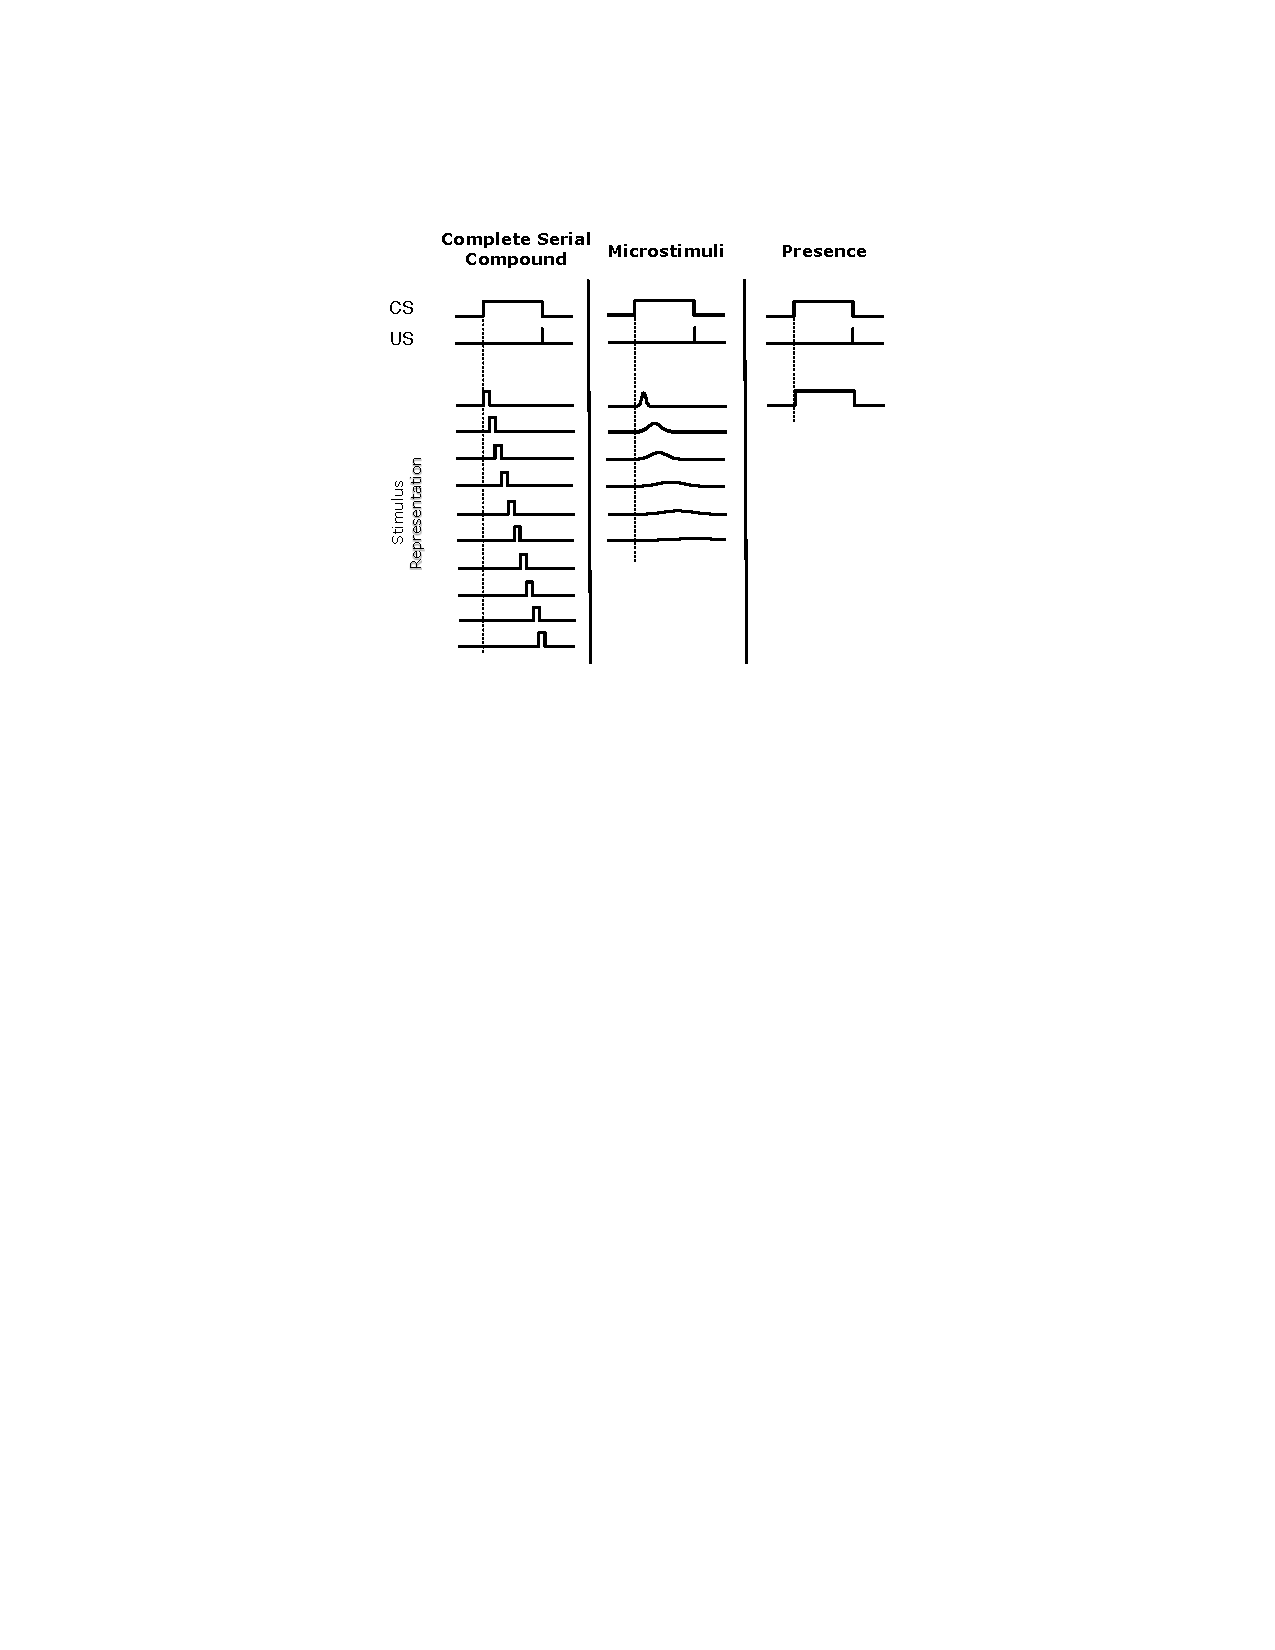
\includegraphics[width=0.5\linewidth]{chap11/fig_11_1}
	\caption{\textit{时间差分}模型有时使用三种刺激表示(列中)。
		每行代表刺激表示的一个元素。
		这三种表示沿时间泛化梯度变化,在完整序列复合(左列)的附近时间点之间没有泛化,在存在表示(右列)的附近时间点之间没有完全泛化。
		微刺激表示占据了中间位置。时间泛化程度决定了学习\textit{非条件刺激}预测的时间粒度。
		改编自学习与行为的微小变化,《评估经典条件反射的TD模型》,第40卷,2012年,第311页,E.A.Ludvig,R.S.Sutton,E.J.Kehoe。经施普林格许可。  \label{fig:11_1}}
\end{figure}

图~\ref{fig:11_1}~所示的最简单表示是图右列中的存在表示。
这种表示对于试验中存在的每个组成\textit{条件刺激}都有一个单一的特征,每当该成分存在时,该特征的值为1,否则为0。
存在表示并不是关于刺激如何在动物大脑中表示的现实假设,但正如我们下面描述的,具有这种表示的\textit{时间差分}模型可以产生经典条件反射中看到的许多时间现象。


对于CSC表示(图14.1的左栏),每个外部刺激的开始都会引发一系列精确定时的短期内部信号,直到外部刺激结束。
这就像假设动物的神经系统有一个时钟,在刺激呈现期间保持精确的时间轨迹;这就是工程师所说的分接延迟线。
“像存在表示一样,CSC表示作为大脑内部如何表示刺激的假设是不现实的,但Ludvig等人(2012)称之为有用的操作”,因为它可以揭示\textit{时间差分}模型在相对不受刺激表示约束时如何工作的细节。
CSC表示也用于大多数\textit{时间差分}模型中对大脑中产生多巴胺的神经元的研究,这是我们在第15章中讨论的主题。
CSC表示通常被视为\textit{时间差分}模型的重要组成部分,尽管这种观点是错误的。



\textit{微刺激}表示(图~\ref{fig:11_1}~的中列)类似于CSC表示,因为每个外部刺激都会引发一系列内部刺激,但在这种情况下,内部刺激(微刺激)并不是这种有限且不重叠的形式;
它们会随着时间的推移而延长并重叠。
随着刺激开始后时间的推移,不同的微刺激集变得或多或少活跃,并且随后的每个微刺激在时间上逐渐变宽并达到较低的最大水平。
当然,根据微刺激的性质,有许多\textit{微刺激}表示的变体,并且在文献中已经研究了许多\textit{微刺激}表示的例子,在某些情况下,还提出了动物大脑如何产生它们的假设(参见本章末尾的书目和历史评论)。
\textit{微刺激}表示比存在或CSC表示作为关于刺激的神经表示的假设更现实,并且它们允许\textit{时间差分}模型的行为与动物实验中观察到的更广泛的现象集合相关。
特别是,通过假设微刺激的级联是由\textit{非条件刺激}和\textit{条件刺激}发起的,并且通过研究微刺激,资格迹和折扣之间相互作用对学习的重要影响,\textit{时间差分}模型有助于构建假设来解释许多经典条件反射的微妙现象以及动物大脑如何产生这些现象。
下面我们将对此进行更多讨论,特别是在第15章中,我们将讨论强化学习和神经科学。


然而,即使使用简单的存在表示,\textit{时间差分}模型也能产生\textit{雷斯科拉-瓦格纳模型}所解释的经典条件反射的所有基本特性,以及超出试验级模型范围的条件反射特征。
例如,正如我们已经提到的,经典条件反射的一个显着特征是,\textit{非条件刺激}通常必须在中性刺激开始后开始进行条件反射,并且在条件反射后,\textit{条件反射}在\textit{非条件刺激}出现之前开始。
换句话说,条件反射通常需要一个积极的\textit{刺激间距},\textit{条件反射}通常会预测\textit{非条件刺激}。
条件反射的强度(例如,\textit{条件刺激}引起的\textit{条件反射}的百分比)如何取决于不同物种和反应系统的\textit{刺激间距}差异很大,但它通常具有以下特性:对于零\textit{刺激间距}或负\textit{刺激间距},即当\textit{非条件刺激}开始与\textit{条件刺激}开始同时发生或早于\textit{条件刺激}开始时,它可以忽略不计(尽管研究发现关联强度有时会略有增加或与负\textit{刺激间距}呈负相关);
它在调节最有效的正\textit{刺激间距}处增加到最大值;
然后在响应系统变化很大的时间间隔后,它会减小到零。
\textit{时间差分}模型的这种依赖性的精确形状取决于其参数的值和刺激表示的细节,但这些\textit{刺激间距}依赖性的基本特征是\textit{时间差分}模型的核心属性。


关于序列复合条件反射,即一个复合\textit{条件刺激}的组成部分按顺序发生的\textit{条件反射},出现的理论问题之一是远程关联的促进作用。
研究发现,如果\textit{条件刺激}和\textit{非条件刺激}之间的空迹线间隔被第二个\textit{条件刺激}填充以形成序列复合刺激,那么第一个\textit{条件刺激}的\textit{条件反射}会得到促进。
图~\ref{fig:11_2}~显示了\textit{时间差分}模型在这种实验的模拟中的行为,该实验的时间细节显示在图的顶部。与实验结果一致(Kehoe,1982),该模型显示由于存在第二个\textit{条件刺激},第一个\textit{条件刺激}的\textit{条件反射}率和\textit{条件反射}的极限水平都得到了促进。

\begin{figure}[!htb]
	\centering
	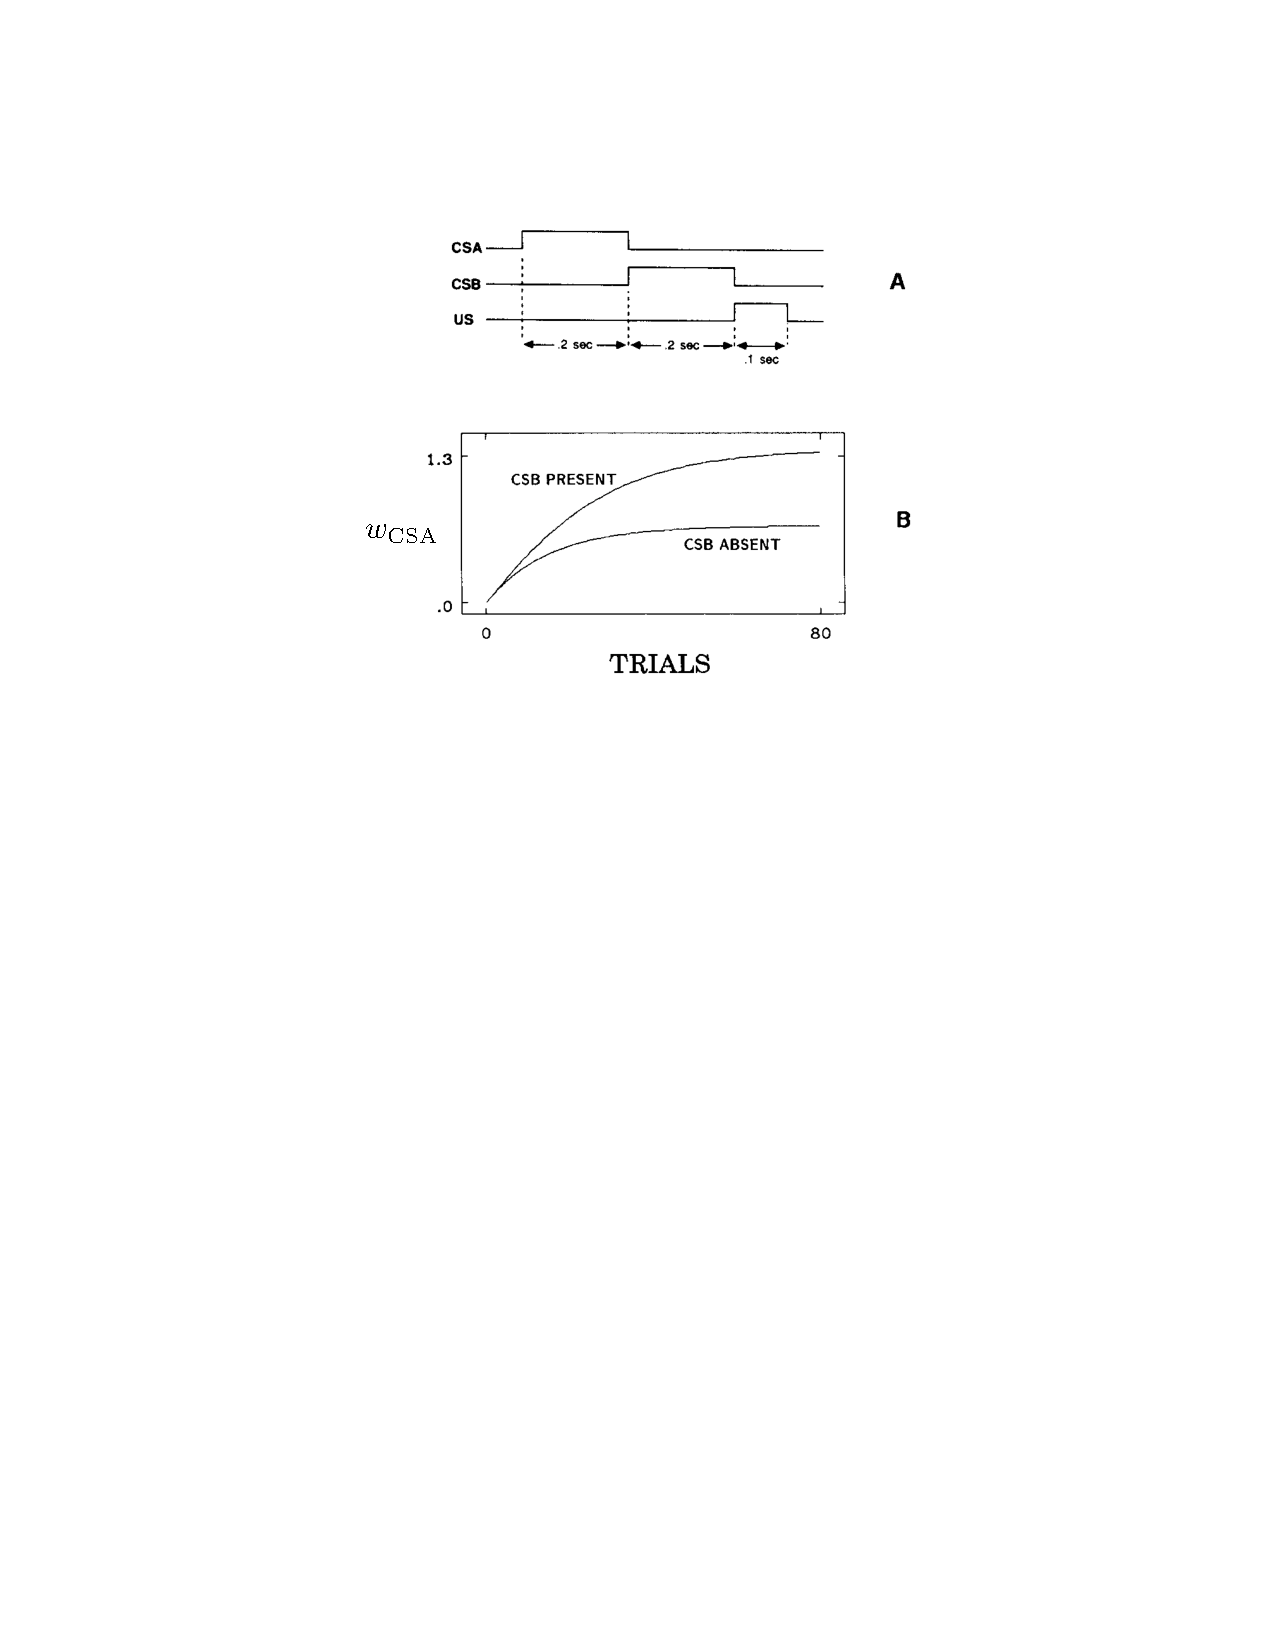
\includegraphics[width=0.5\linewidth]{chap11/fig_11_2}
	\caption{通过\textit{时间差分}模型中的干预刺激促进远程关联。
		上图:试验中刺激之间的时间关系。
		下图:当CSA以上图所示的序列复合形式呈现时,CSA的关联强度在试验的行为,以及当CSA与\textit{非条件刺激}呈现相同的时间关系但没有CSB时的行为。
		改编自Sutton和Barto(1990)。  \label{fig:11_2}}
\end{figure}


Egger和Miller(1962)的一项实验证明了试验中刺激之间时间关系的调节作用,该实验涉及延迟配置中的两个重叠\textit{条件刺激},如图~\ref{fig:11_3}~顶部所示。
尽管CSB与\textit{非条件刺激}的时间关系更好,但与不存在CSA的对照组相比,CSA的存在大大减少了对CSB的\textit{条件反射}。
图~\ref{fig:11_3}~的底部面板显示了\textit{时间差分}模型在使用存在表示的实验模拟中产生的相同结果。

\begin{figure}[!htb]
	\centering
	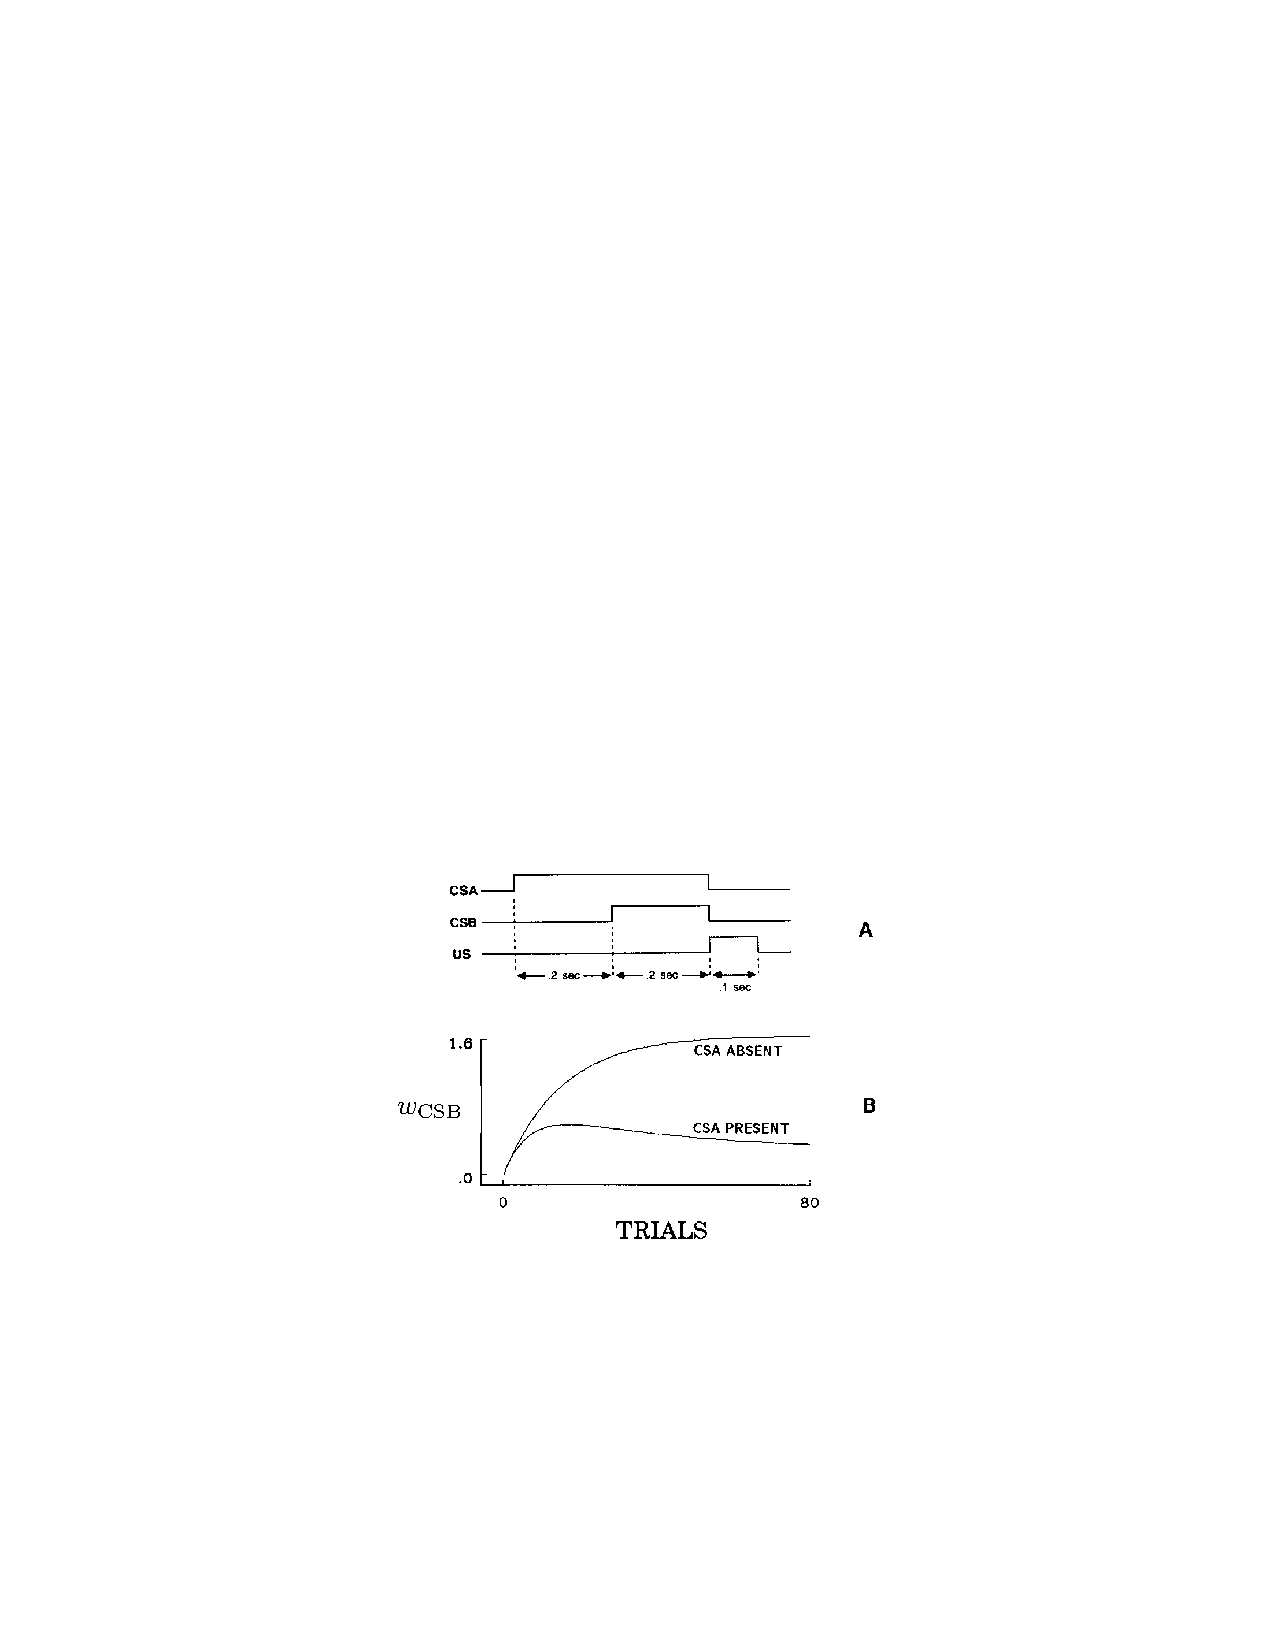
\includegraphics[width=0.5\linewidth]{chap11/fig_11_3}
	\caption{在\textit{时间差分}模型中的Egger-Miller或首位效应。
		上图:试验中刺激之间的时间关系。
		下图:当CSB有或没有CSA时,CSB的关联强度行为。
		改编自Sutton和Barto(1990)。  \label{fig:11_3}}
\end{figure}


\textit{时间差分}模型解释了阻塞现象,因为它是一种纠错的学习规则,就像\textit{雷斯科拉-瓦格纳模型}一样。
然而,除了解释基本的阻塞结果外,\textit{时间差分}模型还预测(使用存在表示和更复杂的表示)如果将阻塞的刺激提前,使其在阻塞刺激之前开始,那么这种阻塞就会被逆转。
\textit{时间差分}模型行为的这一特征值得关注,因为在引入模型时尚未观察到。
回想一下,在阻塞现象中,如果动物已经学会了一个\textit{条件刺激}预测\textit{非条件刺激},那么学习到新添加的第二个\textit{条件刺激}也预测\textit{非条件刺激}会大大减少,即被阻塞。
但是,如果新添加的第二个\textit{条件刺激}比预训练的\textit{条件刺激}更早开始,那么根据\textit{时间差分}模型,对新添加的\textit{条件刺激}的学习不会被阻止。
事实上,随着训练的继续,新添加的\textit{条件刺激}获得了关联强度,而预训练的\textit{条件刺激}失去了关联强度。
\textit{时间差分}模型在这些条件下的行为如图~\ref{fig:11_4}~所示。
该模拟实验与图~\ref{fig:11_3}~的Egger-Miller实验不同之处在于,后者先对较短的\textit{条件刺激}进行训练,直到它与\textit{非条件刺激}完全相关。
这一令人惊讶的预测促使Kehoe,Schreurs和Graham(1987)使用经过充分研究的兔切口膜制剂进行实验。
他们的结果证实了模型的预测,他们指出非\textit{时间差分}模型在解释其数据方面有相当大的困难。


\begin{figure}[!htb]
	\centering
	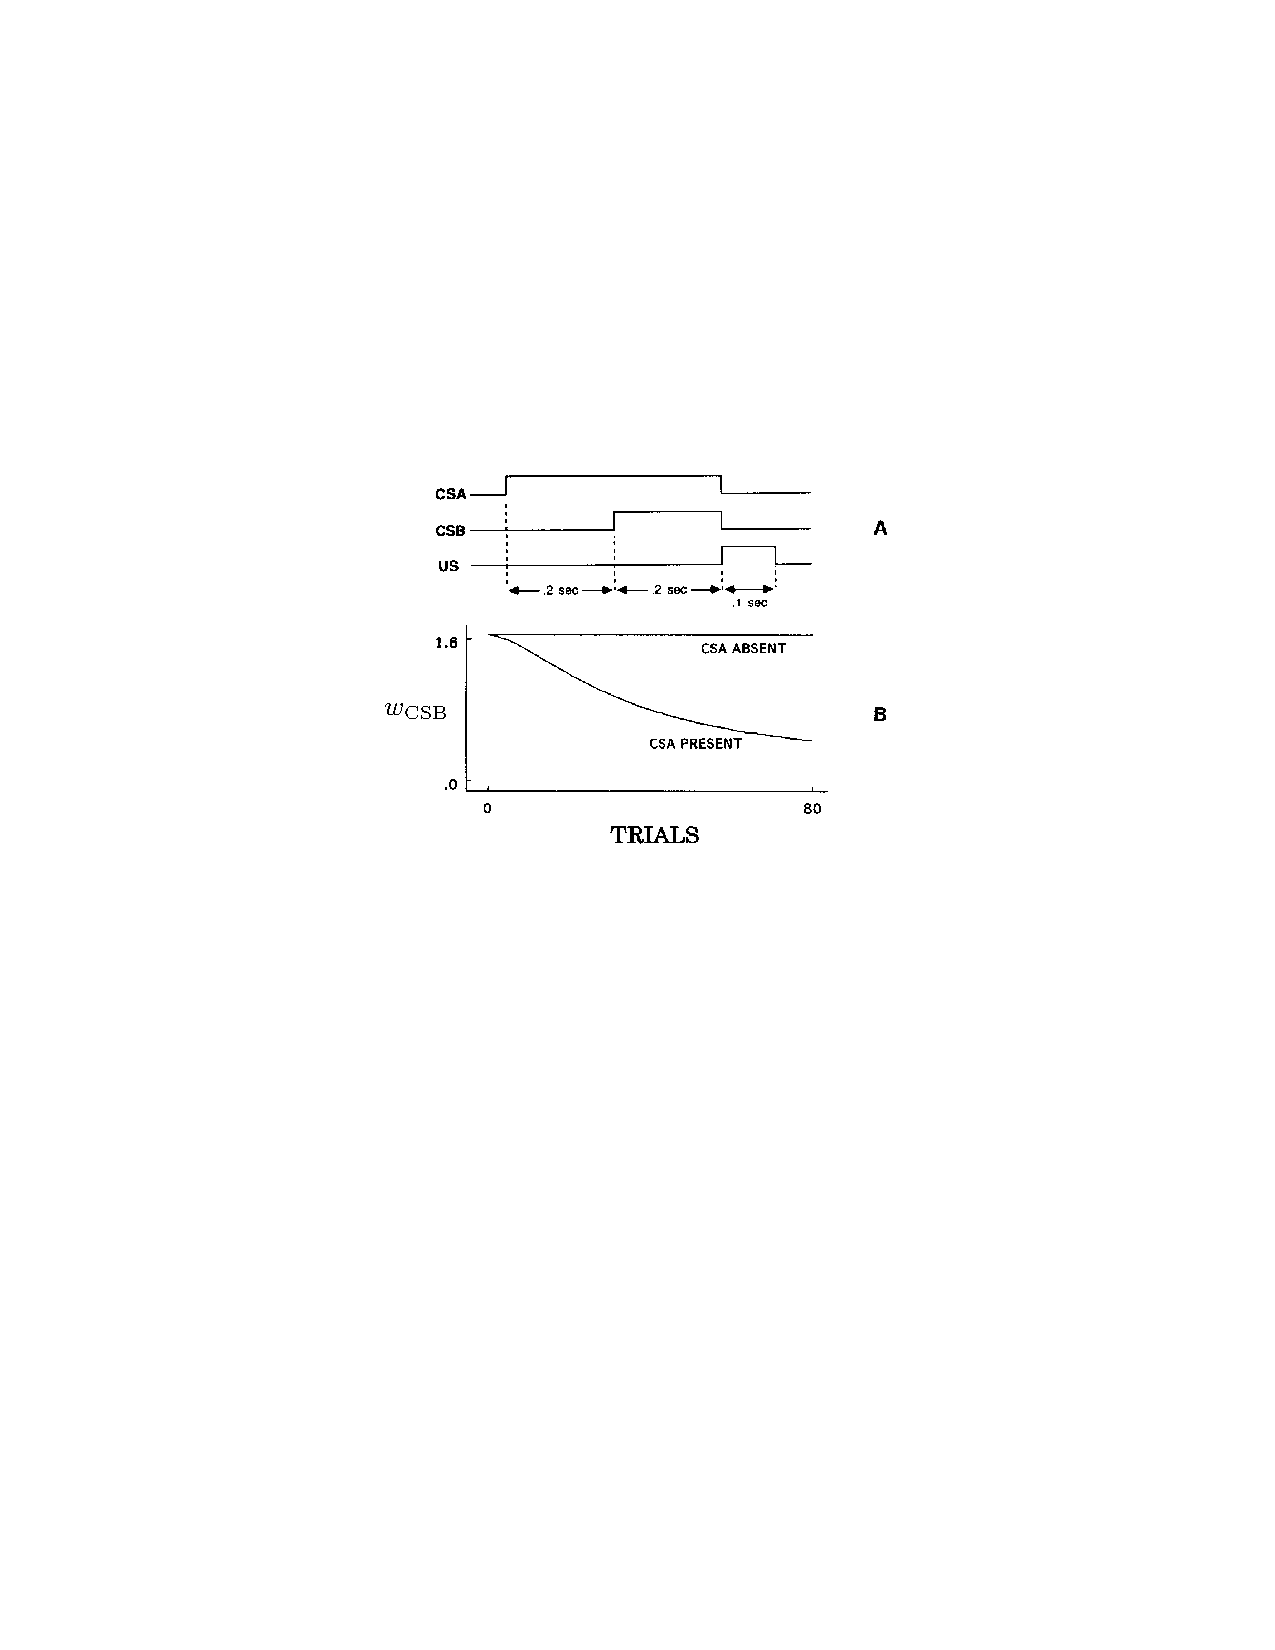
\includegraphics[width=0.5\linewidth]{chap11/fig_11_4}
	\caption{\textit{时间差分}模型中,时间优先覆盖阻塞现象。
		上图:刺激之间的时间关系。
		下图:当CSB有或没有CSA时,CSB的关联强度试验的行为。
		该模拟与图14.3所示的唯一不同之处在于,这里CSB开始完全条件化,CSB的关联强度最初设置为1.653,即CSB单独用于80次试验时达到的最终水平,如图14.3中的“CSA缺席”情况。
		改编自Sutton和Barto(1990)。 \label{fig:11_4}}
\end{figure}


对于\textit{时间差分}模型,较早的预测刺激优先于较晚的预测刺激,因为与本书中描述的所有预测方法一样,\textit{时间差分}模型基于回溯或自举的思想:关联强度的更新将特定状态下的强度转移到较晚状态下的强度。
自举的另一个结果是\textit{时间差分}模型提供了高阶条件反射的解释,这是一种超出了\textit{雷斯科拉-瓦格纳模型}和类似模型的范围的经典条件反射的特征。
如上所述,高阶条件反射是指先前条件反射的\textit{条件刺激}可以充当\textit{非条件刺激}来条件化另一个最初中性的刺激的现象。
图~\ref{fig:11_5}~显示了\textit{时间差分}模型(同样使用存在表示)在高阶\textit{条件反射}实验中的行为,在这种情况下是二阶条件反射。
在第一阶段(图中未显示),CSB被训练来预测\textit{非条件刺激},以便其关联强度增加,这里达到1.6。
在第二阶段,在没有\textit{非条件刺激}的情况下,CSA与CSB配对,顺序排列如图顶部所示。
即使CSA从未与\textit{非条件刺激}配对,它也会获得关联强度。
随着持续的训练,CSA的关联强度达到峰值,然后下降,因为二次强化物CSB的关联强度降低,从而失去了提供二次强化的能力。
CSB的关联强度降低,因为\textit{非条件刺激}在这些高阶条件试验中没有发生。
这些是CSB的消退试验,因为它与\textit{非条件刺激}的预测关系被破坏,因此其作为强化物的能力下降。
在动物实验中也可以看到同样的模式。
在高阶\textit{条件反射}试验中,条件强化的消退使得很难证明高阶\textit{条件反射},除非通过偶尔插入一阶试验定期刷新原始预测关系。


\begin{figure}[!htb]
	\centering
	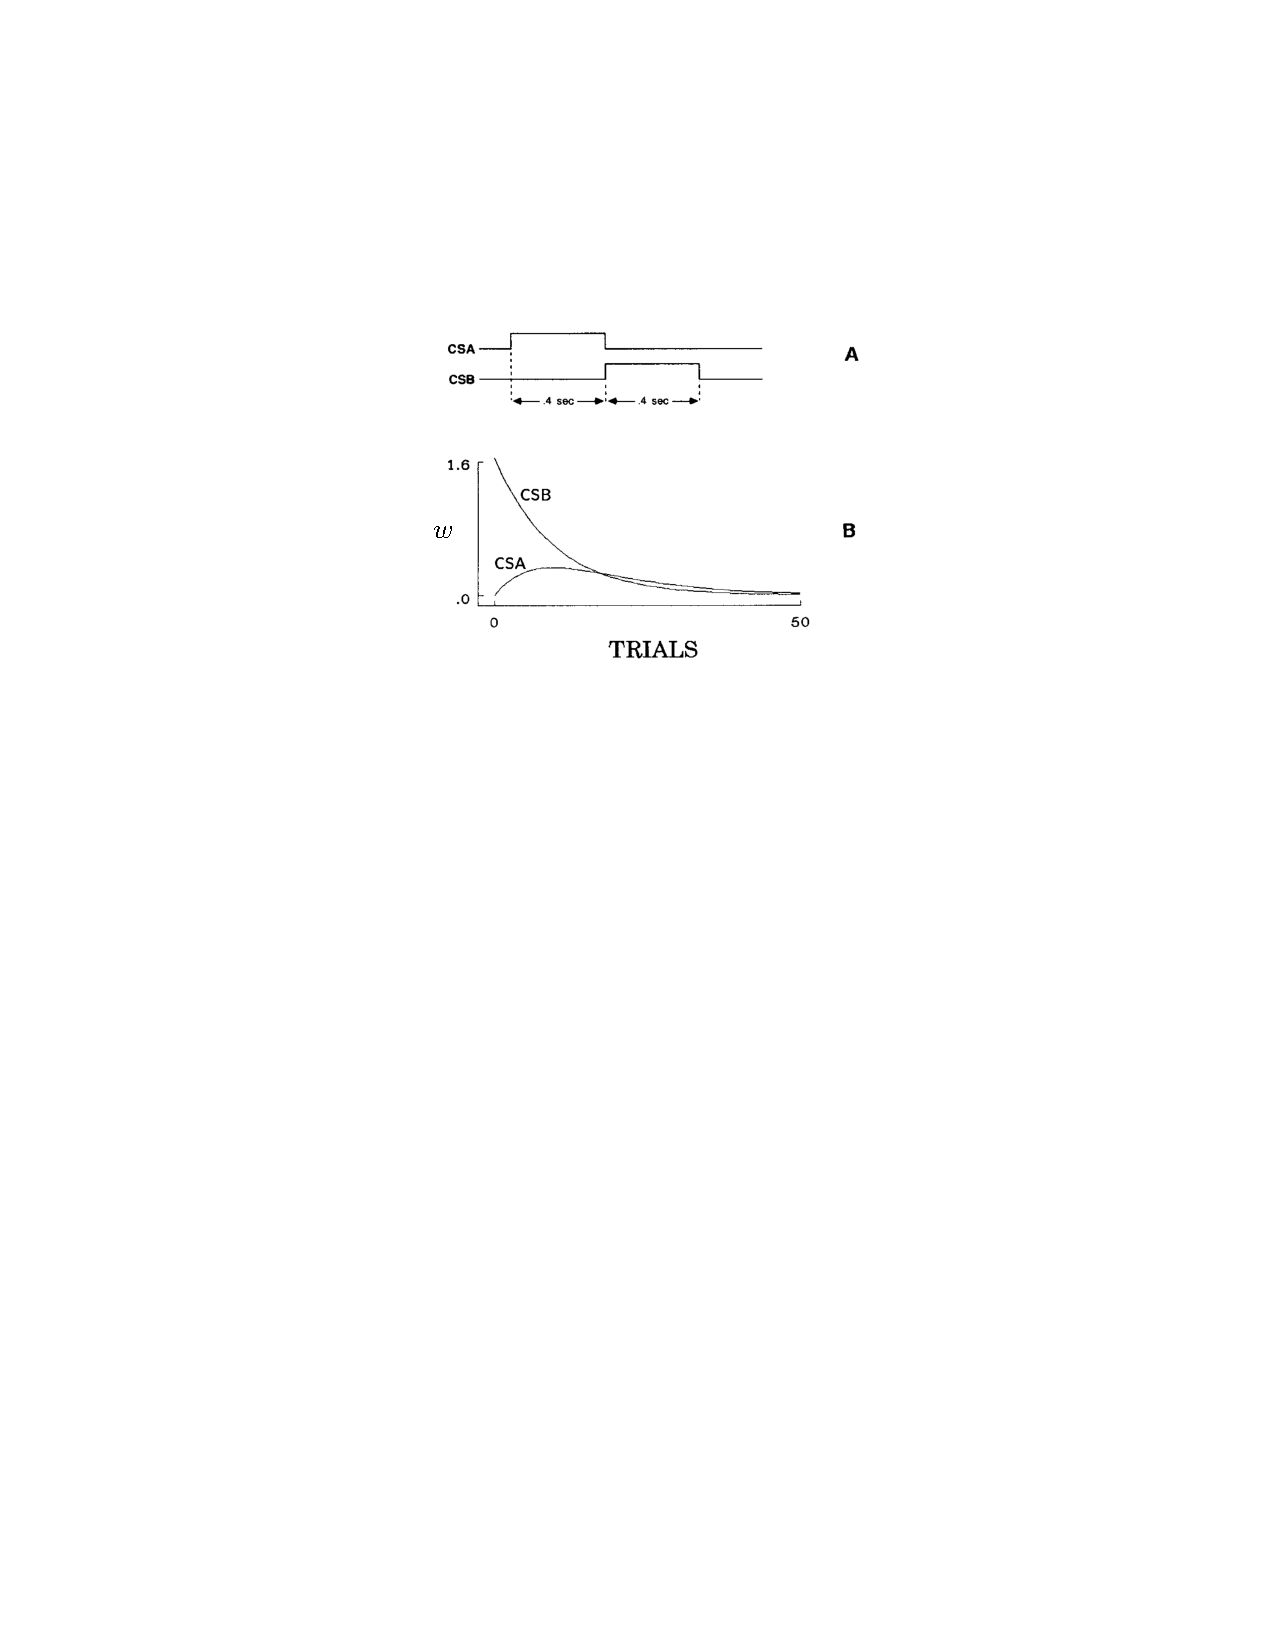
\includegraphics[width=0.5\linewidth]{chap11/fig_11_5}
	\caption{\textit{时间差分}模型的二阶\textit{条件反射}。
		上图:刺激之间的时间关系。
		下图:与CSA和CSB相关的关联强度在试验中的行为。
		第二个刺激CSB在模拟开始时的初始关联强度为1.653\cite{sutton1990integrated}。
	 \label{fig:11_5}}
\end{figure}


\textit{时间差分}模型产生了二阶和高阶条件反射的类似现象,因为$\gamma\hat v(S_{t+1},w_t)$-$\hat v(S_t,w_t)$出现在\textit{时间差分}错误$\delta t$(14.5)中。这意味着作为先前学习的结果,$\gamma\hat v(S_{t+1},w_t)$可以与 $\hat v(S_t,w_t)$不同,使得$\delta t$非零(时间差异)。这种差异与(14.5)中的$R_{t+1}$具有相同的状态,这意味着就学习而言,时间差异和\textit{非条件刺激}的发生之间没有区别。
事实上,\textit{时间差分}算法的这一特征是其发展的主要原因之一,我们现在通过第6章所述的与动态规划的联系来理解它。自举值与二阶和高阶条件反射密切相关。


在上述\textit{时间差分}模型行为的示例中,我们仅检查了\textit{条件刺激}组成部分的关联强度的变化;
我们没有研究该模型对动物\textit{条件反射}特性的预测:其时间、形状以及它们如何发展过度条件反射试验。
这些特性取决于物种、观察到的反应系统以及\textit{条件反射}试验的参数,但在许多不同动物和不同反应系统的实验中,\textit{条件反射}的幅度或\textit{条件反射}的概率随着\textit{非条件刺激}的预期时间的接近而增加。
例如,在我们上面提到的兔子的切口膜反应的经典\textit{条件反射}中,随着\textit{条件反射}试验的进行,从\textit{条件刺激}开始到切口膜开始穿过眼睛的延迟在试验中减少,并且这种预期闭合的幅度在\textit{条件刺激}和\textit{非条件刺激}之间的间隔内逐渐增加,直到膜在\textit{非条件刺激}的预期时间达到最大闭合。
这种\textit{条件反射}的时间和形状对于其适应性意义至关重要,过早覆盖眼睛会降低视力(即使切口膜是半透明的),而太晚覆盖它几乎没有保护价值。
对于经典\textit{条件反射}模型来说,捕获这样的\textit{条件反射}特征具有挑战性。


\textit{时间差分}模型不包括任何将\textit{非条件刺激}预测的时间过程$\hat v(S_t,w_t)$转换为可以与动物\textit{条件反射}特性进行比较的过程的机制。
最简单的选择是让模拟\textit{条件反射}的时间过程等于\textit{非条件刺激}预测的时间过程。
在这种情况下,模拟\textit{条件反射}的特征及其在试验中的变化方式仅取决于所选的刺激表示以及模型参数$\alpha$、$\gamma$和$\lambda$的值。


图~\ref{fig:11_6}~显示了学习过程中不同时间点\textit{非条件刺激}预测的时间过程,图~\ref{fig:11_1}~中显示了三种表示。
在这些模拟中,\textit{非条件刺激}在\textit{条件刺激}开始后发生了25个时间步出现,并且$\alpha$=0.05、$\gamma$=0.95和$\lambda$=0.97。使用CSC表示(图~\ref{fig:11_6}~左),\textit{时间差分}模型形成的\textit{非条件刺激}预测曲线在\textit{条件刺激}和\textit{非条件刺激}之间的整个间隔内呈指数增长,直到它在\textit{非条件刺激}发生时达到最大值(在第25个时间步)。
这种指数增长是\textit{时间差分}模型学习规则中折扣的结果。对于存在表示(图~\ref{fig:11_6}~中),当刺激存在时,\textit{非条件刺激}的预测几乎是恒定的,因为每个刺激只有一个权重或关联强度需要学习。
因此,具有存在表示的\textit{时间差分}模型不能重建\textit{条件反射}时间的许多特征。
使用\textit{微刺激}表示(右图~\ref{fig:11_6}),\textit{时间差分}模型的\textit{非条件刺激}预测的发展更加复杂。
经过200次试验后,预测的曲线是用CSC表示产生的\textit{非条件刺激}预测曲线的合理近似值。


\begin{figure}[!htb]
	\centering
	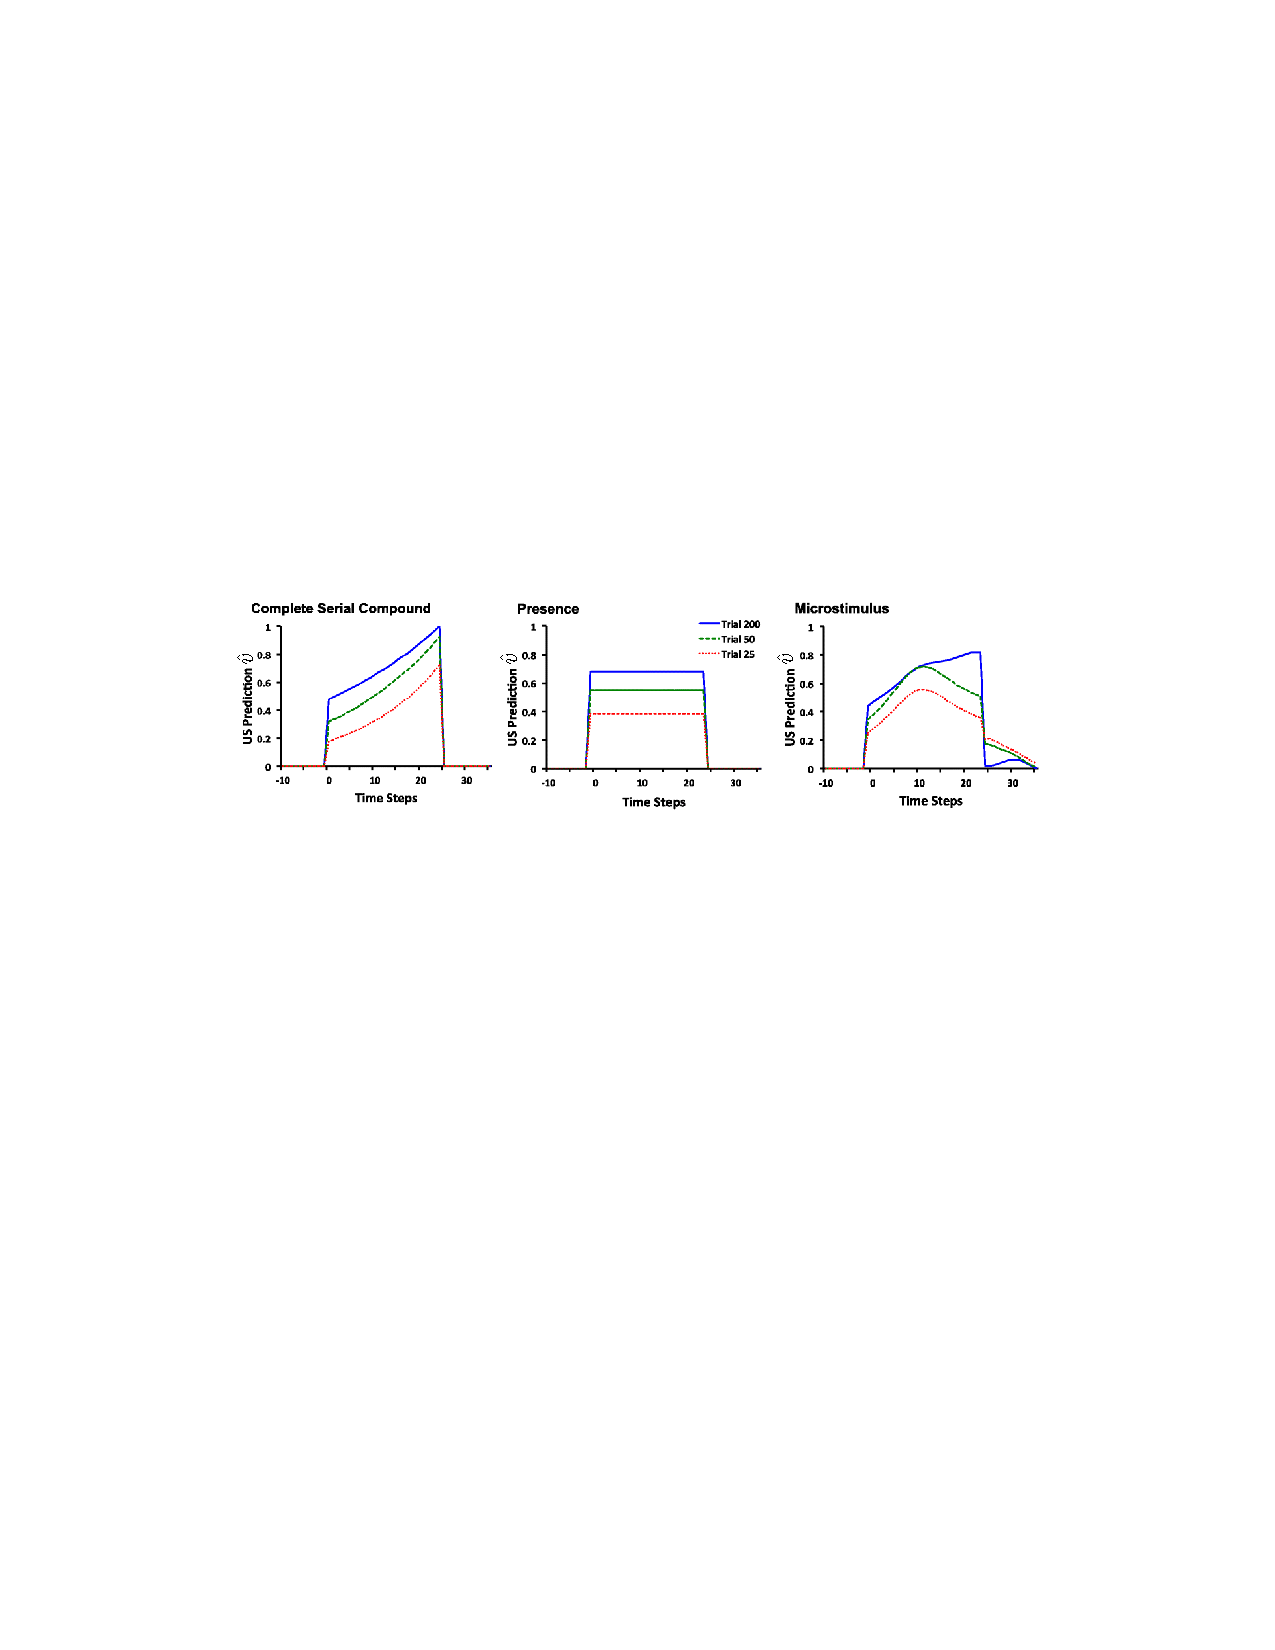
\includegraphics[width=0.8\linewidth]{chap11/fig_11_6}
	\caption{具有三种不同刺激表示的\textit{时间差分}模型在获取过程中\textit{非条件刺激}预测的时间过程。
		左:对于完整序列复合(CSC),\textit{非条件刺激}预测在整个间隔内呈指数增长,并且在\textit{非条件刺激}出现时达到峰值。
		在极限情况下(第200次试验),\textit{非条件刺激}预测在\textit{非条件刺激}强度达到峰值(这些模拟中为1)。
		中间:通过存在表示,\textit{非条件刺激}的预测收敛到几乎恒定的水平。
		这个恒定水平由\textit{非条件刺激}强度和\textit{条件刺激}-\textit{非条件刺激}间隔的长度决定。
		右:使用微刺激表示,在极限情况下,\textit{时间差分}模型通过不同微刺激的线性组合近似于CSC表示下的指数增长的时间过程。\label{fig:11_6}}
\end{figure}


图~\ref{fig:11_6}~所示的\textit{非条件刺激}预测曲线并不是为了精确匹配\textit{条件反射}在任何特定动物实验中条件作用过程中产生的曲线,但它们说明了刺激表示对从\textit{时间差分}模型得出的预测的强烈影响。
此外,尽管我们只能在这里提到,但刺激表现如何与折扣和资格迹相互作用,对于确定\textit{时间差分}模型产生的\textit{非条件刺激}预测曲线的性质很重要。
我们在这里可以讨论的另一个方面是不同响应生成机制的影响,这些机制将\textit{非条件刺激}预测转化为\textit{条件反射}曲线;
图~\ref{fig:11_6}~所示的曲线是“原始的”\textit{非条件刺激}预测曲线。
即使没有任何关于动物大脑如何从\textit{非条件刺激}预测中产生明显反应的特殊假设,但是,图~\ref{fig:11_6}~中CSC和\textit{微刺激}表示的曲线随着\textit{非条件刺激}时间的接近而增加,并在\textit{非条件刺激}时间达到最大值,正如许多动物条件作用实验所见。


\textit{时间差分}模型与特定的刺激表征和反应产生机制相结合,能够解释动物经典条件反射实验中观察到的令人惊讶的广泛现象,但它远不是一个完美的模型。
为了生成经典条件作用的其他细节,需要扩展模型,也许可以通过添加基于模型的元素和自适应调整其某些参数的机制来实现。
建模经典条件反射的其他方法与\textit{雷斯科拉-瓦格纳模型}风格的误差校正过程明显不同。
例如,贝叶斯模型在概率框架内工作,经验可以修改概率估计。
所有这些模型都有助于我们理解经典条件反射。


也许\textit{时间差分}模型最显着的特点是它基于一种理论,即我们在本书中描述的理论,该理论提出了动物的神经系统在经历条件反射时试图做的事情:
它试图形成准确的长期预测,与刺激表现方式和神经系统如何工作所施加的限制相一致。
换句话说,它提出了经典条件反射的规范性解释,其中长期而不是即时的预测是一个关键特征。


经典条件作用的\textit{时间差分}模型的发展就是一个例子,其中明确的目标是模拟动物学习行为的一些细节。
因此,\textit{时间差分}学习除了作为一种算法,也是这种生物学习方面模型的基础。
正如我们在第~\ref{chap:chap12}~章中所讨论的,\textit{时间差分}学习也被证明是产生多巴胺的神经元活动的基础模型,多巴胺是哺乳动物大脑中的一种化学物质,与奖励处理密切相关。
在这些例子中,强化学习理论与动物行为和神经数据进行了详细的联系。


我们现在转向考虑强化学习和动物行为在工具性条件作用实验中的对应关系,这是动物学习心理学家研究的另一种主要类型的实验室实验。


\section{操作性条件反射} \label{sec:instrumental_conditioning}

在工具性条件反射实验中,学习依赖于行为的后果:强化刺激的传递取决于动物的行为。
相比之下,在经典的条件反射实验中,强化刺激-“\textit{非条件刺激}”是独立于动物的行为而传递的。
工具性条件反射通常被认为与操作性条件反射相同,术语是为行为依赖性强化实验引入的\cite{skinner2019behavior},尽管使用这两个术语的人的实验和理论在许多方面有所不同,其中一些我们将在下面讨论。
我们将专门使用工具性条件反射这个术语来描述那些强化取决于行为的实验。
工具性条件反射的根源可以追溯到\textit{非条件刺激}心理学家\textit{爱德华$\cdot$李$\cdot$桑代克}在本书第一版出版前100年进行的实验。


\textit{桑代克}观察到猫被放在迷箱中时的行为,“它们可以通过适当的动作从迷箱中逃生”(图~\ref{fig:11_7}~)。
例如,猫可以通过执行三个独立的动作来打开一个盒子的门:
按下盒子后面的平台,用爪子拉绳子,然后上下推一根推杆。
当第一次放在迷箱中,外面可以看到食物时,除了少数几只\textit{桑代克}的猫外,所有猫都表现出“明显的不适迹象”和“异常剧烈的活动,本能地努力逃离困境”\cite{thorndike1898animal}。


\begin{figure}[!htb]
	\centering
	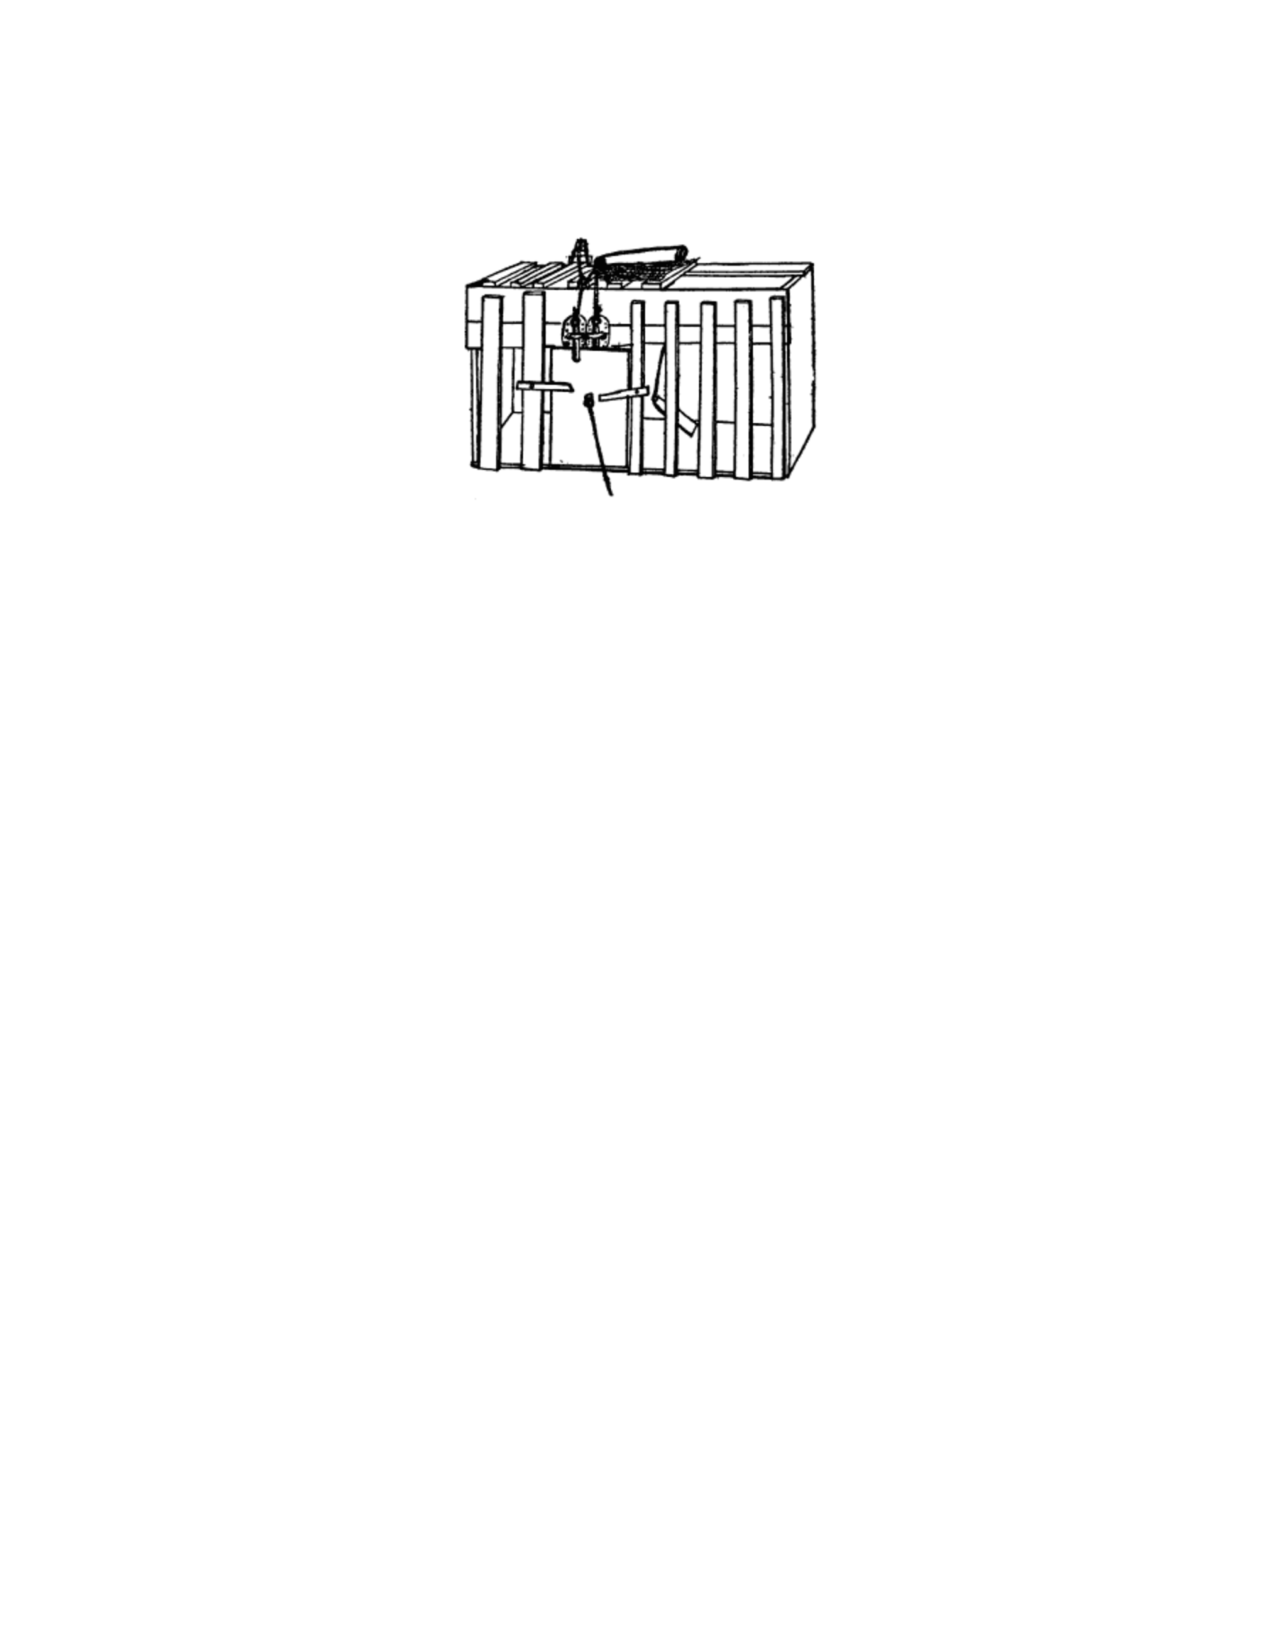
\includegraphics[width=0.5\linewidth]{chap11/fig_11_7}
	\caption{\textit{桑代克}的一个迷箱\cite{thorndike1898animal}。  \label{fig:11_7}}
\end{figure}

在对不同的猫和具有不同逃生机制的盒子进行的实验中,\textit{桑代克}记录了每只猫在每个盒子中多次逃生所花费的时间。
他观察到,时间几乎总是随着经验的增加而减少,例如从300秒减少到6或7秒。
他这样描述猫在箱子里的行为:


在冲动的挣扎中,一只猫在盒子上抓来抓去,它很可能会抓住绳子、环或按钮来开门。
渐渐地,所有其他不成功的冲动都会被消除,而导致成功行为的特定冲动会因随之而来的愉悦感而被强化,直到经过多次尝试后,猫被放入盒子后,会立即以一种明确的方式抓住按钮或环\cite{thorndike1898animal}。


这些和其他实验(一些是使用狗,小鸡,猴子,甚至鱼)导致\textit{桑代克}制定了许多学习的“定律”,其中最有影响力的是效果律,我们在第一章中引用过的一个版本。
这条定律描述了通常所说的通过试错学习。
如第1章所述,效果律的许多方面都产生了争议,多年来其细节有所修改。
尽管如此,这种法则以某种形式表达了一种持久的学习原则。


强化学习算法的基本特征对应于效果律描述的动物学习特征。
首先,强化学习算法是选择性的,意味着它们会尝试替代方案,并通过比较其结果来进行选择。
其次,强化学习算法是关联性的,这意味着通过选择找到的替代方案与特定情况或状态相关联,以形成智能体的策略。
就像效果律描述的学习一样,强化学习不仅是发现产生大量奖励的行为的过程,而且是将这些行为与情境或状态联系起来的过程。
\textit{桑代克}使用“选择和连接”这个短语来描述学习。
进化中的自然选择是选择过程的一个主要例子,但它不是关联的(至少正如人们普遍理解的那样);
监督学习是关联的,但它不是选择的,因为它依赖于直接告诉智能体如何改变行为的指令。


从计算的角度来看,效果律描述了一种将搜索和记忆结合起来的基本方法:
在每种情况下,以尝试和选择许多动作的形式进行搜索,并以将情景与迄今为止发现的行为联系起来的关联形式进行记忆,以便在这些情况下发挥最佳作用。
搜索和记忆是所有强化学习算法的重要组成部分,无论记忆是以智能体的策略、价值函数还是环境模型的形式出现。


强化学习算法需要进行搜索,意味着它必须以某种方式进行探索。
动物显然也是如此,与早期的动物学习研究人员对动物在\textit{桑代克}的迷箱中选择行为的指导程度存在分歧。
行动是绝对随机、盲目摸索的结果吗?(Woodworth,1938,第777页),还是有某种程度的指导,是来自先前的学习、推理还是其他手段?
尽管包括\textit{桑代克}在内的一些思想家似乎采取了前一种立场,但其他人则倾向于更深思熟虑的探索。
强化学习算法允许智能体在选择动作时可以使用多少指导有很大的自由度。
我们在本书中介绍的算法中使用的探索形式,如$\epsilon$贪婪和上置信界动作选择,只是最简单的探索方法之一。
更复杂的方法是可能的,唯一的要求是必须有某种形式的探索才能使算法有效工作。



我们处理强化学习的特点是允许随时可用的一组动作取决于环境的当前状态,这与\textit{桑代克}在他的猫的迷箱行为中观察到的情况相呼应。
猫从它们在当前情况下本能表现的行为中选择动作,\textit{桑代克}称之为“本能冲动”。
“首先放在一个迷箱中,猫会本能地抓挠和咬,用力进行挣扎:
这是猫在发现自己被困在狭小空间时的本能反应。
成功的动作是从这些行为中选择的,而不是从每一个可能的动作或活动中选择。
这就像我们形式主义的特征,从一个状态$ s $中选择的动作属于一组可接受的动作 $ A(s) $。
指定这些动作是强化学习的一个重要方面,因为它可以从根本上简化学习。
它们就像动物的本能冲动。
另一方面,\textit{桑代克}的猫可能是根据一种特定于动作的本能动作排序进行探索的,而不仅仅是从一组动作中进行选择。
这是使强化学习更容易的另一种方法。


克拉克$\cdot$赫尔\cite{skinner2019behavior}是受效果律影响最大的动物学习研究人员之一。
他们研究的核心是根据行为结果选择行为的理念。
强化学习与赫尔理论有着共同的特征,其中包括类似资格的机制和二次强化,以解释在动作与随后的强化刺激之间存在显著的时间间隔时学习的能力(见第~\ref{sec:delayed_reinforcement}~节)。
随机性也在赫尔的理论中发挥了作用,他称之为“行为振荡”来引入探索行为。


斯金纳并不完全认同效果律的记忆方面。他反对关联联结的概念,而是强调从自发产生的行为中进行选择。
他引入“操作性”一词来强调动作对动物环境影响的关键作用。
与\textit{桑代克}等人的实验不同,斯金纳的操作性条件反射实验允许动物受试者长时间不间断地行为。
他发明了操作性条件反射箱,现在称为“斯金纳箱”,其中最基本的版本包含一个杠杆或按钮,动物可以按下它来获得奖励,如食物或水,这些奖励将根据一个明确的规则(称为强化程序)进行发放。
通过记录杠杆按压的累积次数作为时间的函数,斯金纳和他的追随者可以研究不同强化程序对动物杠杆按压速度的影响。
使用我们在本书中介绍的强化学习原理对类似实验的建模结果并不完善,但我们在本章末尾的书目和历史评论部分提到了一些例外。


斯金纳的另一个贡献来自于他认识到通过强化逐步逼近目标行为来训练动物的有效性,他称之为塑造过程。
虽然这项技术已经被包括斯金纳本人在内的其他人使用过,但当他和同事试图训练鸽子用喙推木球时,这项技术的重要性给他留下了深刻的印象。
在等待了很长时间而没有看到任何可以强化推球行为后,他们


…决定强化任何与推球有相似的反应,也许一开始只是看球的行为,然后选择更接近最终形式的反应。结果令我们惊讶不已。
几分钟后,球在盒子的墙上弹来弹去,就像鸽子是壁球冠军一样\cite{skinner1958reinforcement}。


鸽子不仅学会了一种对鸽子来说不寻常的行为,而且还通过一个互动过程快速学会了,在这个过程中,它的行为和强化条件相互响应。
斯金纳将改变强化条件的过程比作雕塑家将粘土塑造成理想形状的工作。
塑造也是计算强化学习系统的强大技术。
当一个\textit{智能体}很难接收到任何非零奖励信号时,无论是由于奖励情况的稀疏性还是由于初始行为的不可接近性,从一个更容易的问题开始,随着\textit{智能体}的学习逐渐增加其难度可能是一种有效的,有时是必不可少的策略。


心理学中一个与工具性条件反射特别相关的概念是动机,它指的是影响行为方向和活力(或活力)的过程。
例如,\textit{桑代克}的猫就有动力逃离迷箱,因为它们想要得到外面的食物。
实现这一目标对他们来说是有益的,并加强了允许他们逃跑的行动。
很难将具有多个维度的动机概念精确地与强化学习的计算观点联系起来,但它与某些维度有明确的联系。


从某种意义上说,强化学习\textit{智能体}的奖励信号是其动机的基础:
从长远来看,\textit{智能体}的动机是最大化其获得的总奖励。
因此,动机的一个关键方面是,是什么使\textit{智能体}的经验获得回报。
在强化学习中,奖励信号取决于强化学习\textit{智能体}的环境状态和\textit{智能体}的行为。
此外,正如第1章所指出的,\textit{智能体}环境的状态不仅包括关于机器外部的信息,如包括\textit{智能体}的生物体或机器人,还包括机器内部的信息。
一些内部状态成分对应于心理学家所说的动物的动机状态,这会影响对动物的奖励。
例如,一只动物饥饿时吃东西比刚吃完一顿令人满意的饭时会得到更多的回报。
状态依赖的概念足够广泛,可以对奖励信号的生成产生多种类型的调节影响。


价值函数进一步与心理学家的动机概念相联系。
如果选择行动的最基本动机是获得尽可能多的奖励,那么对于使用价值函数选择行动的强化学习\textit{智能体}来说,更直接的动机是沿着其价值函数的梯度上升,即选择预期会导致最有价值的下一个状态的行动(或者本质上相同的事情,选择具有最大行动价值的行动)。
对于这些\textit{智能体}来说,价值函数是决定其行为方向的主要驱动力。


动机的另一个维度是,动物的动机状态不仅影响学习,而且影响动物学习后的行为强度或活力。
例如,学会在迷宫的目标箱中找到食物后,饥饿的老鼠比不饥饿的老鼠跑得更快。
这种动机方面与我们在这里介绍的强化学习框架没有那么紧密的联系,但在本章末尾的书目和历史评论部分,我们引用了几篇基于强化学习的行为活力理论的出版物。


现在我们转向讨论当强化刺激在其强化的事件发生后很久才出现时的学习。
强化学习算法使用的机制能够通过延迟强化进行学习(资格迹和\textit{时间差分}学习),与心理学家关于动物在这些条件下如何学习的假设密切相关。


\section{延迟强化} \label{sec:delayed_reinforcement}


\textit{效果律}要求对连接进行逆向影响,一些早期的批评者无法理解现在如何能够影响过去的事情。
这种担忧加剧了这样一个事实,即当行动与随之而来的奖励或惩罚之间存在相当大的延迟时,学习仍然可以发生。
同样,在经典条件反射中,当\textit{非条件刺激}出现时间与\textit{条件刺激}结束时间之间存在不可忽略的时间间隔时,学习仍然可以发生。
我们称之为延迟强化问题,这与\textit{明斯基}\cite{minsky1961steps}所称的学习系统的信用分配问题有关:如何在可能涉及成功的许多决策中分配成功的信用?
本书中介绍的强化学习算法包括两种解决此问题的基本机制。
第一种是使用资格迹,第二种是使用\textit{时间差分}方法学习价值函数,这些价值函数可以提供近乎即时的行为评估(在工具性反射实验等任务中),或提供即时的预测目标(在经典条件反射实验等任务中)。
这两种方法都对应于动物学习理论中提出的类似机制。


巴甫洛夫(1927)指出,每个刺激都必须在刺激结束后的一段时间内在神经系统中留下痕迹,他提出,当\textit{条件刺激}结束和\textit{非条件刺激}出现之间存在时间间隔时,刺激痕迹使学习成为可能。
直到今天,在这些条件下的条件反射被称为痕迹条件反射(第285页)。
假设当\textit{非条件刺激}到达时,\textit{条件刺激}的痕迹仍然存在,学习是通过痕迹和\textit{非条件刺激}的同时存在而发生的。
我们在第15章讨论了一些关于神经系统痕迹机制的建议。


刺激痕迹也被提议作为一种手段,用于桥接动作与随之而来的奖惩之间的时间间隔。
例如,在赫尔的内在学习理论中,“整体刺激痕迹”解释了他所谓的动物的目标梯度,即工具性条件反应的最大强度如何随着强化延迟的增加而降低\cite{hull1932goal,hull1943principles}。
赫尔假设动物的动作会留下内部刺激,其痕迹会随着时间呈指数衰减。
根据当时可用的动物学习数据,他假设痕迹在30到40秒后有效地趋于零。




本书中描述的算法中使用的资格迹线类似于赫尔迹线:它们是过去状态访问或过去状态-动作对的衰减迹线。
资格迹线是由Klopf\cite{klopf1972brain}在他的神经元理论中引入的,在他的神经元理论中,它们是突触中过去活动的时间扩展迹线,即神经元之间的连接。
Klopf的迹线比我们算法使用的指数衰减迹线更复杂,当我们在第~\ref{sec:hedonistic_neurons}~节中学习他的理论时,我们会对此进行更多讨论。


为了解释比刺激痕迹跨越更长时间的目标梯度,\textit{赫尔}\cite{hull1943principles}提出,更长的梯度是由从目标向后传递的条件强化产生的,这一过程与他的整体刺激痕迹一起起作用。
动物实验表明,如果条件有利于在延迟期间发展条件性强化,那么学习不会像在阻碍二次强化的条件下那样随着延迟的增加而减少。
如果在延迟间隔期间有规律发生的刺激,则有条件的强化是有利的。
然后,似乎奖励实际上并没有延迟,因为有更即时的条件强化。
因此,赫尔设想基于刺激痕迹调节的初级强化的延迟存在一个初级梯度,并且通过条件性强化逐渐修改和延长。


本书中提出的算法使用资格迹和价值函数来实现延迟强化学习,这与赫尔关于动物在这些条件下如何学习的假设相对应。
\textit{行动者}第~\ref{sec:neural_ac}~节和第~\ref{sec:ac_rules}~节中讨论的\textit{评论家}体系结构最清楚地说明了这种对应关系。
\textit{评论家}使用\textit{时间差分}算法学习与系统当前行为相关的值函数,即预测当前策略的回报。
参与者根据\textit{评论家}的预测更新当前策略,或者更准确地说,根据\textit{评论家}预测的变化更新当前策略。
\textit{评论家}产生的\textit{时间差分}误差充当了参与者的条件强化信号,即使主要奖励信号本身被大大延迟,也能立即评估性能。
估计动作值函数的算法,例如Q学习和Sarsa,类似地使用\textit{时间差分}学习原理,通过条件强化来实现延迟强化学习。
我们在第15章中讨论的\textit{时间差分}学习与产生多巴胺的神经元的活动之间的紧密联系,为强化学习算法与赫尔学习理论这一方面的联系提供了进一步支持。


\section{认知地图} \label{sec:cognitive_maps}

基于模型的强化学习算法使用的环境模型与心理学家所称的认知图具有共同的元素。
回想对规划和学习的讨论,环境模型指的是\textit{智能体}可以用来预测其环境在状态转换和奖励方面如何响应其行为的任何东西,而规划指的是从这样的模型计算策略的任何过程。
环境模型由两部分组成:状态转换部分编码了关于行为对状态变化的影响的知识,奖励模型部分编码关于每个状态或每个状态-动作对预期的奖励信号的知识。
基于模型的算法通过使用模型来选择动作,以根据未来状态和预期从这些状态产生的奖励信号来预测可能的行为过程的后果。
最简单的规划是比较“想象”决策序列集合的预测后果。


关于动物是否使用环境模型的问题,如果是这样的话,模型是什么样的,它们是如何学习的,在动物学习研究的历史上起着至关重要的作用。
一些研究人员通过展示潜在学习,挑战了当时流行的\textit{刺激反应}学习观和行为观,这与最简单的无模型学习策略相对应。
在最早的潜在学习实验中,两组老鼠在迷宫中跑步。
对于实验组来说,在实验的第一阶段没有奖励,但在第二阶段开始时食物突然被引入迷宫的目标箱中。
对于对照组来说,食物在两个阶段都在目标箱中。
问题是,在没有食物奖励的情况下,实验组的老鼠在第一阶段是否会学习到任何东西。
尽管实验老鼠在没有奖励的阶段似乎学习不多,但他们一发现第二阶段引入的食物,就迅速赶上了对照组的老鼠。
得出的结论是,“在非奖励期,实验组的老鼠他们正在开发一种潜在的迷宫学习方法,一旦引入奖励,他们就能够利用这种方法”\cite{blodgett1929effect}。



潜在学习与心理学家\textit{爱德华$\cdot$托尔曼}以及其他类似的人联系最为密切,\textit{爱德华$\cdot$托尔曼}将这一结果解释为动物可以在没有奖励或惩罚的情况下学习环境的认知地图,并且当他们有动机达到目标时,他们可以稍后使用该地图\cite{tolman1948cognitive}。
认知地图还可以让老鼠规划通往目标的路线,这与老鼠在最初探索中使用的路线不同。
对这些结果的解释导致了心理学中行为主义/认知二分法核心的持久争议。
现代意义上,认知地图不仅限于空间布局模型,更普遍的是环境模型或动物的“任务空间”模型\cite{wilson2014orbitofrontal}。
潜在学习实验的认知图解释类似于动物使用基于模型的算法的说法,并且即使没有明确的奖励或惩罚也可以学习环境模型。
然后,当动物受到奖励或惩罚的激励时,模型被用于规划。


\textit{托尔曼}对动物如何学习认知图的描述是,它们通过在探索环境时经历刺激的连续性来学习刺激-刺激(或S-S)关联。
在心理学中,这被称为期望理论:给定S-S关联,刺激的发生会产生对下一个刺激的期望。
这很像控制工程师所说的系统识别,即从标记的训练示例中学习具有未知动力学的系统模型。
在最简单的离散时间版本中,训练示例是S-$S'$对,其中$S$是状态,$S'$是后续状态。
当观察到s时,模型会创建期望接下来将观察$S'$。对计划更有用的模型也涉及动作,因此示例类似于SA-$S'$,其中当动作$ A $在状态$ S $下执行时,$ S' $是预期的。
了解环境如何产生回报也很有用。在这种情况下,例子是S-$ R $或SA-$ R $的形式,其中$ R $是与$ S $或SA对相关联的奖励信号。
这些都是监督学习的形式,通过这些形式,\textit{智能体}可以获得类似认知的地图,无论它在探索其环境时是否接收到任何非零奖励信号。


\section{习惯性和目标导向的行为} \label{sec:habitual_behavior}

无模型和基于模型的强化学习算法之间的区别对应于心理学家对学习行为模式的习惯性和目标导向控制之间的区别。
习惯是由适当的刺激触发的行为模式,然后或多或少地自动执行。
根据心理学家如何使用这个短语,目标导向行为是有目的的,因为它受目标价值以及行为与其后果之间关系的知识的控制。
习惯有时被认为是由先前的刺激控制的,而目标导向的行为被认为是由其后果控制的\cite{dickinson1980contemporary,dickinson1985actions}。
目标导向控制的优点是,当环境改变对动物行为的反应方式时,它可以迅速改变动物的行为。
虽然习惯行为对习惯环境的输入反应迅速,但它无法快速适应环境的变化。
目标导向行为控制的发展可能是动物智力进化的一个重大进步。


图~\ref{fig:11_8}~说明了无模型和基于模型的决策策略在假设任务中的差异,在该任务中,老鼠必须在具有独特目标框的迷宫中导航,每个目标框都提供了所示数量级的相关奖励(图~\ref{fig:11_8}~顶部)。
从$ S_1 $开始,老鼠必须首先选择左(L)或右(R),然后必须在$ S_2 $或$ S_3 $再次选择L或R才能到达其中一个目标框。
目标框是老鼠情节任务每一集的终端状态。无模型策略(图~\ref{fig:11_8}~左下)依赖于状态-动作对的存储值。
这些动作值(Q值)是对老鼠从每个(非终点)状态采取的每个动作所能预期的最高回报的估计值。
它们是通过多次从开始到结束运行迷宫的试验获得的。
当动作值对最佳回报的估计足够好时,老鼠只需在每个状态下选择动作值最大的动作即可做出最佳决策。
在这种情况下,当动作值估计足够准确时,老鼠从$ S_1 $中选择L,从$ S_2 $中选择R,以获得4的最大回报。
另一种不同的无模型策略可能仅仅依赖于缓存的策略而不是动作值,从而实现从$ S_1 $到L以及从$ S_2 $到R的直接链接。
在这两种策略中,决策都不依赖于环境模型。
不需要参考状态转换模型,目标框的功能与它们提供的奖励之间也不需要连接。


图~\ref{fig:11_8}(右下)说明了基于模型的策略。它使用由状态转换模型和奖励模型组成的环境模型。
状态转换模型显示为决策树,奖励模型将目标框的独特特征与每个目标框中要找到的奖励相关联。
(与状态$ S_1 $,$ S_2 $和$ S_3 $相关的奖励也是奖励模型的一部分,但这里它们是零,没有显示。)
基于模型的\textit{智能体}可以通过使用模型来模拟行动选择序列来决定在每个状态下转向哪种方式,以找到产生最高回报的路径。
在这种情况下,回报是从路径末尾的结果中获得的奖励。
在这里,使用足够精确的模型,老鼠将选择L,然后选择R以获得4的奖励。
比较模拟路径的预测收益是一种简单的规划形式,可以通过第8章讨论的多种方式完成。


当无模型\textit{智能体}的环境改变其对\textit{智能体}行为的反应方式时,\textit{智能体}必须在改变的环境中获得新的经验,在此期间可以更新其策略和/或价值函数。
例如,在图~\ref{fig:11_8}(左下)所示的无模型策略中,如果其中一个目标框以某种方式转变为提供不同的奖励,则老鼠将不得不穿过迷宫,可能需要多次才能在到达目标框时体验新的奖励,同时根据此经验更新其策略或其行动价值函数(或两者)。
关键的一点是,对于一个无模型的\textit{智能体}来说,要改变其策略为一个状态指定的动作,或者改变与一个状态相关的动作值,它必须移动到该状态,从该状态开始动作,可能多次,并经历其动作的后果。


\begin{figure}[!htb]
	\centering
	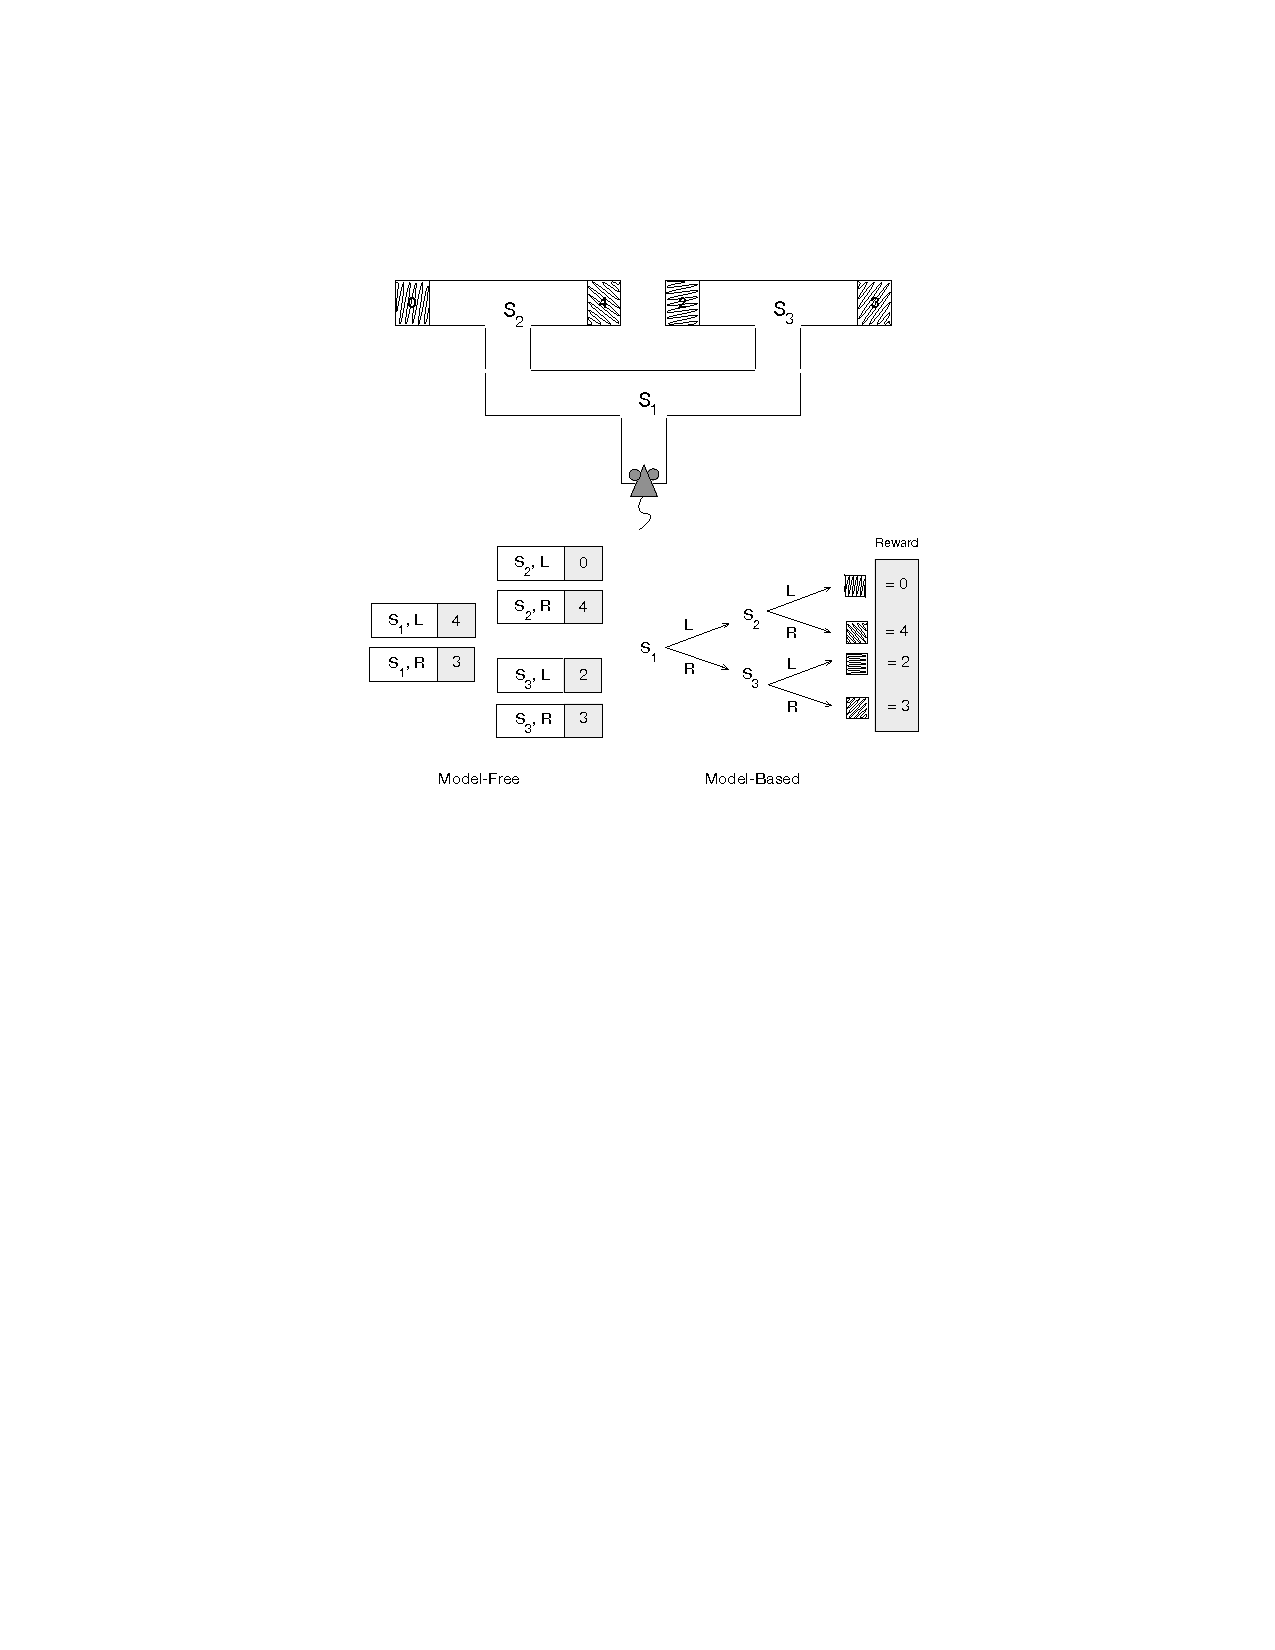
\includegraphics[width=0.65\linewidth]{chap11/fig_11_8}
	\caption{基于模型和无模型的策略来解决假设的顺序动作选择问题。
		上图:一只老鼠穿越迷宫,迷宫中有独特的目标框,每个目标框都有一个显示值的奖励。
		左下:无模型策略依赖于在许多学习试验中获得的所有状态动作对的存储动作值。
		为了做出决策,老鼠只需在每个状态下选择该状态动作值最大的动作。
		右下:在基于模型的策略中,老鼠学习一个环境模型,该模型由状态-动作-下一个状态转换的知识和一个奖励模型组成,该奖励模型由与每个独特目标框相关的奖励知识组成。
		老鼠可以通过使用该模型模拟动作选择的序列来决定在每个状态下转向哪种方式,从而找到产生最高回报的路径。
		\label{fig:11_8}}
\end{figure}


基于模型的\textit{智能体}可以适应其环境的变化,而不需要这种“个人经验”来了解变化所影响的状态和行为。
模型的更改(通过计划)会自动更改其策略。规划可以确定环境变化的后果,而这些变化在\textit{智能体}自己的经历中从未联系在一起。
例如,再次参考图~\ref{fig:11_8}~中的迷宫任务,想象一只具有先前学习的转移和奖励模型的老鼠直接放置在$ S_2 $右侧的目标框中,那里可用的奖励现在具有值1而不是4。
即使不涉及在迷宫中找到目标框所需的行动选择,老鼠的奖励模型也会改变。规划过程将使新的奖励知识对迷宫运行产生影响,而不需要额外的迷宫经验;
在这种情况下,在$ S_1 $和$ S_3 $处将策略更改为右转,以获得3的回报。


这种逻辑正是动物结果贬值实验的基础。
这些实验的结果提供了一个洞察动物是否已经养成了一种习惯,或者它的行为是否处于目标导向的控制之下。
结果贬值实验类似于潜在的学习实验,因为奖励从一个阶段变为下一个阶段。
在学习的初始奖励阶段之后,结果的奖励值会发生变化,包括变为零甚至负值。


\textit{亚当斯}\cite{adams1981instrumental}进行了这种类型的早期重要实验。
他们通过工具性条件反射训练老鼠,直到老鼠在训练箱中使劲按压杠杆以获取蔗糖颗粒。然后将老鼠放在同一个箱子中,将杠杆收回,并允许它们非依赖性地获取食物,这意味着颗粒可以独立于它们的动作提供给它们。
在自由获取这些颗粒15分钟后,一组老鼠注射了引起恶心的有毒氯化锂。
重复三次,最后一次注射的老鼠都没有吃任何非依赖性的颗粒,这表明颗粒的奖励价值降低了,颗粒贬值了。
在一天后的下一个阶段,将老鼠再次放置在箱子中,并进行一段时间的消退训练,这意味着响应杆回到原位但与颗粒分配器断开连接,因此按下它不会释放颗粒。
问题是,即使没有经历由于杠杆按压而贬值的奖励,那些颗粒奖励值降低的老鼠是否会比没有颗粒奖励值降低的老鼠杠杆按压更少。
事实证明,从消退试验一开始,注射了毒药的老鼠的反应率就显著低于未注射的老鼠。


\textit{亚当斯}和\textit{迪克森}得出结论,注射的老鼠通过将杠杆按压与颗粒、颗粒与恶心联系起来的认知图,将杠杆按压与随之而来的恶心联系起来。
因此,在消退试验中,老鼠“知道”按下杠杆的后果是他们不想要的,因此他们从一开始就减少了杠杆的按压。
重要的是,他们减少了杠杆的按压,而没有经历过杠杆的按压直接伴随着生病:生病时没有杠杆。
他们似乎能够将行为选择的结果(按下杠杆之后会得到颗粒)的知识与结果的奖励值(颗粒是要避免的)结合起来,因此可以相应地改变他们的行为。
并不是每个心理学家都同意这种实验的认知解释,这不是解释这些结果的唯一可能的方法,而是模型基于规划的解释被广泛接受。


没有什么可以阻止\textit{智能体}同时使用无模型算法和基于模型的算法,并且有充分的理由同时使用这两种算法。
我们从自己的经验中知道,如果重复足够多,目标导向的行为往往会变成习惯性行为。实验表明,这种情况也发生在老鼠身上。
\textit{亚当斯}\cite{adams1982variations}进行了一项实验,以观察长期训练是否会将目标导向的行为转变为习惯性行为。
他通过比较经历不同训练量的老鼠结果贬值的影响来做到这一点。
如果与接受较少训练的老鼠相比,延长训练使老鼠对贬值的敏感性降低,这将证明延长训练使行为更加习惯。
亚当斯的实验紧跟着刚刚描述的亚当斯\cite{adams1981instrumental}的实验。
简单点说,一组老鼠接受训练,直到他们做出100次奖励杠杆按压,另一组老鼠(过度训练组)接受训练,直到他们做出500次奖励杠杆按压。
训练后,两组老鼠的颗粒奖励值均降低(使用氯化锂注射)。
然后对两组老鼠进行一次消退训练。亚当斯的问题是,贬值是否会使过度训练的老鼠的杠杆按压率低于非过度训练的老鼠,这将证明延长训练会降低对结果贬值的敏感性。
结果表明,贬值大大降低了非过度训练老鼠的杠杆按压率。
相反,对于过度训练的老鼠来说,贬值对他们的杠杆按压几乎没有影响;事实上,如果有什么不同的话,它会使它更有活力。
(完整的实验包括对照组,表明不同程度的训练本身并没有显着影响学习后的杠杆按压率。)
这一结果表明,虽然非过度训练的老鼠以目标导向的方式行事,对他们的行为结果的知识敏感,但过度训练的老鼠已经养成了杠杆按压的习惯。



从计算的角度来看这个结果和其他类似的结果,可以洞察为什么人们可能期望动物在某些情况下表现出习惯性行为,在其他情况下以目标导向的行为,以及为什么它们在学习的过程中会从一种控制模式转变为另一种控制模式。
虽然动物无疑使用的算法与我们在本书中介绍的算法并不完全匹配,但可以通过考虑各种强化学习算法所暗示的权衡来深入了解动物行为。
计算神经科学家Daw\cite{daw2005uncertainty}提出的一个想法是,动物同时使用无模型和基于模型的过程。
每个流程都会提出一个行动,而选择执行的行动是由流程提出的,该流程被认为是两个流程中更值得信赖的一个,这是由整个学习过程中保持的置信度度量所决定的。
在早期学习中,基于模型的系统的规划过程更值得信赖,因为它将短期预测联系在一起,与无模型过程的长期预测相比,短期预测可以在经验较少的情况下变得准确。
但随着经验的不断积累,无模型过程变得更加可信,因为由于模型不准确和使规划可行所采取的捷径而出错(例如各种形式的树剪枝:删除不希望的搜索树分支)。根据这个想法,随着经验的积累,人们预计会从目标导向的行为转变为习惯性行为。
关于动物如何在目标导向和习惯性控制之间进行仲裁,已经提出了其他观点,并且行为学和神经科学研究都在继续研究这一问题和相关问题。


无模型算法和基于模型的算法之间的区别被证明对这项研究很有用。
人们可以在抽象设置中检查这些类型算法的计算含义,这些抽象设置揭示了每种类型的基本优点和局限性。
这既有助于提出问题,也有助于尖锐化问题,从而指导实验设计,这对于提高心理学家对习惯性和目标导向行为控制的理解是必要的。


\section{总结}

本章的目的是讨论强化学习与心理学中动物学习实验研究之间的对应关系。
我们一开始就强调,本书中描述的强化学习并不是为了模拟动物行为的细节。
它是一个抽象的计算框架,从人工智能和工程的角度探索理想情况。
但许多基本的强化学习算法都受到心理学理论的启发,在某些情况下,这些算法有助于开发新的动物学习模型。
本章描述了这些对应关系中最引人注目的部分。


预测算法和控制算法在强化学习方面的区别类似于动物学习理论在经典或巴甫洛夫条件反射和工具条件反射之间的区别。
操作条件反射实验和经典条件反射实验之间的关键区别在于,前者的强化刺激取决于动物的行为,而后者则不然。
通过\textit{时间差分}算法学习预测对应于经典条件反射,我们描述了\textit{时间差分}模型的经典条件反射,这是强化学习原理解释了动物学习行为某些细节的一个实例。
该模型通过包含影响学习中个体试验中事件的时间维度来概括了影响\textit{雷斯科拉-瓦格纳模型},并提供了二阶条件反射的说明,即强化刺激的预测者本身成为强化者。
它也是对大脑多巴胺神经元活动的影响观点的基础,我们在第~\ref{chap:chap12}~章中讨论了这一点。


试错学习是强化学习控制方面的基础。
我们介绍了\textit{桑代克}用猫和其他动物进行的实验的一些细节,这些实验导致了他的效果定律,我们在这里和第一章中对此进行了讨论。
我们指出,在强化学习中,探索不一定局限于“盲目摸索”;
只要有一些探索,就可以通过使用先天和先前学习的知识通过复杂方法产生试验。
我们讨论了\textit{斯金纳}称为“塑造”的训练方法,在这种方法中,奖励的条件会逐渐改变,以训练动物逐渐接近期望的行为。
塑造不仅是动物训练必不可少的,也是训练强化学习智能体的有效工具。
这也与动物动机状态的概念有关,动物的动机状态影响动物将要接近或避免什么,以及动物将奖励或惩罚什么事件。


本书中介绍的强化学习算法包括两种解决延迟强化问题的基本机制:资格迹和通过\textit{时间差分}算法学习的值函数。
这两种机制在动物学习理论中都有先例。资格迹类似于早期理论的刺激痕迹,价值函数对应于二次强化在提供几乎即时的评估反馈中的作用。


本章讨论的下一个对应关系是强化学习的环境模型与心理学家所谓的认知图之间的对应关系。
20世纪中期进行的实验旨在证明动物有能力学习认知图,作为状态-动作关联的替代品或补充,并在以后使用它们来指导行为,特别是当环境意外变化时。
强化学习中的环境模型就像认知图,因为它们可以通过监督学习方法学习,而不依赖于奖励信号,然后可以在以后用于规划行为。


强化学习在无模型和基于模型的算法之间的区别对应于习惯性行为和目标导向行为之间的心理学区别。
无模型算法通过访问策略或动作值函数中的信息来做出决策,而基于模型的方法则使用\textit{智能体}环境的模型选择动作作为提前计划的结果。
结果贬值实验提供了有关动物行为是习惯性还是在目标导向控制下的信息。
强化学习理论有助于澄清对这些问题的思考。


动物学习明显地为强化学习提供了启示,但作为一种机器学习,强化学习旨在设计和理解有效的学习算法,而不是复制或解释动物行为的细节。
我们专注于动物学习的各个方面,这些方面与解决预测和控制问题的方法有着明确的联系,强调了强化学习和心理学之间富有成效的双向思想,而没有深入探讨许多行为细节和争议,这些都占据了动物学习研究人员的注意力。
强化学习理论和算法的未来发展可能会利用与动物学习的许多其他特征的联系,因为这些特征的计算效用得到了更好的认可。
我们期望强化学习和心理学之间的一系列想法将继续为这两个学科带来成果。


强化学习与心理学和其他行为科学领域之间的许多联系超出了本章的范围。
我们在很大程度上忽略了与决策心理学的联系,后者侧重于学习发生后如何选择行动或如何做出决策。
我们也没有讨论生态学家和行为生态学家研究的生态和进化行为方面的联系:动物如何相互关联以及它们的物理环境,以及它们的行为如何促进进化。
优化MDP和动态编程在这些领域中占有重要地位,我们对\textit{智能体}与动态环境交互的强调与复杂“生态”中\textit{智能体}行为的研究有关。
本书中省略的多\textit{智能体}强化学习与行为的社会方面有关。
尽管这里没有涉及这些方面,但强化学习绝不应被解释为排斥进化观点。
强化学习并没有暗示对学习和行为的白板观。
事实上,工程应用的经验突出了将类似于进化为动物提供的知识构建到强化学习系统中的重要性。





